\documentclass[11pt,spanish,listoffigures,listoftables]{tfgetsinf}

\usepackage[utf8]{inputenc} 
\usepackage{listings}
\usepackage{color}
\usepackage{subcaption}
\usepackage{float}

\graphicspath{ {images/} }

% Tex global defintions
\lstdefinestyle{default}{
    frame=tb,
    aboveskip=3mm,
    belowskip=3mm,
    showstringspaces=true,
    showspaces = false,
    columns=flexible,
    basicstyle=\ttfamily\small,
    numbers=none,
    breaklines=true,
    breakatwhitespace=true,
    tabsize=2,
    showspaces = true
}

\lstdefinestyle{python}{
    language=Python,
    numbers=none,
    basicstyle=\ttfamily\small
}
% End text global definitions


\title{Simulación de datos de sensores industriales}
\author{Pedro Henrique Mano Figueiredo Fernandes}
\tutor{Francisco Sánchez Cid}
\curs{2015-2016}

\keywords
{Machine learning, Big Data, PCA} 
{Machine learning, Big Data, PCA}
{Machine learning, Big Data, PCA} 

\begin{document}

% Abstract
\begin{abstract}[spanish]
Los entornos industriales hacen uso de sensores para obtener mediciones de varios factores en su cadena de producción. En las fases iniciales, la cantidad de datos generados es muy reducida, por lo que no es significativa para permitir la aplicación de técnicas de Big Data. Estas técnicas pueden descubrir muchos patrones en los datos, útiles para detección de anomalías o predicción futura. El proyecto descrito en este documento busca simular nuevos datos a través de un pequeña cantidad de datos generados por sensores industriales. La aplicación de estas técnicas se extiende a todo el contexto de proyectos IoT ({\em Internet of Things}), donde los sensores representan la principal fuente de datos. 
\end{abstract}

\begin{abstract}[english]
The industrial environments make use of sensors for acquiring metrics on several variables in their production pipeline. In the initial phases, the generated data has very low volume, making it hard to apply Big Data techniques. These techniques can bring much insight over the data, useful for anomaly detection or future prediction. The project described in this document seeks the simulation of new data using a small amount of data generated by industrial sensors. The application of such techniques can be extended to the entire context of IoT ({\em Internet of Things}), where sensors represent the main source of data.
\end{abstract}

\tableofcontents

\mainmatter

% Introducción
\chapter{Introducción}
Este proyecto tiene como fuente de datos uno o varios sensores de un mecanizado industrial de inyección de plástico. Los sensores efectúan mediciones de varios factores con una regularidad temporal, generando así muestras de datos en determinados intervalos de tiempo. Cuando se trata de sensores, es normal que los datos no tengan la calidad necesaria para aplicar técnicas matemáticas. Hay que tener en cuenta que la frecuencia de las mediciones no es necesariamente constante, que pueden existir interrupciones, ruido y redundancias. Además, en el ámbito de IoT ({\em Internet of Things}), se añade la inherente conectividad de los aparatos como factor de complejidad.

Las técnicas de Big Data, en particular {\em Machine Learning}, necesitan gran cantidad de datos para poder inducir modelos matemáticos que expliquen esos datos. Cuanto más datos mejor, para un aprendizaje más robusto y fiable. Sin embargo, al principio de los proyectos, la cantidad de datos recolectados suele ser pequeña y insuficiente para poder extraer conocimiento significativo de los mismos. El objetivo de este proyecto es aprender y simular el comportamiento de uno o varios sensores a través de una cantidad reducida de datos recolectados en los mismos. 

Una vez preparado el {\em dataset}, es necesario aprender un modelo matemático que lo describa. Las técnicas usadas para ese efecto son del ámbito de {\em Machine Learning}. 

%La fase inicial del análisis es la ingesta de los datos. El dataset proporcionado es de reducida dimensión, tiene tan solo 5MB, por lo que la tarea de ingestión no es intensiva. Sin embargo, hay que tratar los datos en bruto antes de empezar a usarlos. El fichero de datos es de texto, así que hay que hacer determinadas conversiones para poder usar tipos más específicos, como sean fechas y números. El primer problema tiene que ver con los formatos de fecha, que no son correctos para el locale España, lo que exige una adaptación de los algoritmos de parsing.
%Los pasos descritos son muy comunes en análisis de datos y en particular en el {\em pipeline} de Big Data.
    
    \section{Estructura del documento}
    
    Este documento se estructura de la siguiente forma: la descripción del problema; el estado del arte; un análisis sobre el {\em dataset} y respectivas transformaciones para adecuar los datos; las soluciones propuestas y respectiva base teórica; la experimentación, resultados y discusión; conclusiones del trabajo realizado y posibles mejoras; y termina con las fuentes bibliográficas que han servido de base del estudio.

% Descripción del problema
\chapter{Descripción del problema}
El paradigma de IoT ({\em Internet of Things}) tiene mucha presencia en la industria. Se utilizan sensores para controlar determinados factores en las cadenas de producción. Los datos generados son de gran importancia. Con el debido tratamiento y análisis, estos datos pueden ayudar descubrir conocimiento nuevo. En el entorno industrial, ese conocimiento se puede traducir en la anticipación de anomalías o mejoras de rendimiento de las máquinas, con todo el beneficio que eso conlleva.

La extracción de conocimiento de los datos se hace con técnicas estadísticas de {\em Machine Learning}. Estas técnicas están relacionadas con Big Data por la simple regla de que cuantos más datos mejor. Los modelos matemáticos que explican los datos son más robustos si hay mucho volumen de datos. Sin embargo, en las etapas iniciales de implantación de IoT no hay mucha cantidad de datos, lo que dificulta la aplicación de {\em Machine Learning}.

Hay que tener en cuenta que los datos de sensores suelen tener problemas de calidad, sobre todo relacionados con ruido, redundancias o frecuencia de muestro. Por ejemplo, si un sensor mide la temperatura de una máquina, esa medición sufre interferencias del ambiente, por lo que la medición no es completamente objetiva. Ese efecto se conoce por ruido. Cuanto a las redundancias, pueden suceder en casos de pérdida de conectividad, en que el sensor vuelve a dar una métrica aunque la haya dado ya anteriormente. Esto sería, también, un caso de cambio de la frecuencia de muestreo, 	que se traduce en irregularidades de la serie temporal asociada a los datos. 

El objetivo de este proyecto es aprender y simular datos de sensores industriales. Los nuevos datos, de mucho mayor volumen, podrán ser usados para probar y depurar los algoritmos de detección de averías y de predicción desarrollados para entornos Big Data. 

% Estado del Arte
\chapter{Estado del Arte}
Los problemas de ruido y redundancias en los datos son comunes y están bastante estudiados. Para solucionar ese problema, las técnicas de reducción de dimensionalidad, en que los datos son reducidos a lo esencial, suelen tener buenos resultados. PCA ({\em Principal Component Analysis} es la técnica más usual. PCA se usa para descomponer un conjunto de datos multivariante en un grupo de componentes ortogonales que mejor explican la varianza. El ajuste a los datos es de tipo lineal.

Las primeras componentes son las que mayor varianza explican y por eso se llaman principales. El orden de las componentes es relevante, la primera es la más explicativa, la segunda la que más explica quitando la primera, y así sucesivamente. Así que es de esperar que lo que están explicando las últimas sea, realmente, el ruido de la señal. El artículo \textit{A Tutorial on Principal Component Analysis} \cite{shlens} deja patente esa evidencia en el objetivo de filtrar el ruido y redundancias para obtener la dinámica importante de los datos.

Aunque PCA no tenga capacidades de predicción (pertenece a la categoría de {\em unsupervised learning}), se puede usar para simular nuevos datos, como se defiende en el artículo 'The Truth About Principal Component and Factor Analysis'. Aparte de las componentes que explican los datos, PCA obtiene también las proyecciones a lo largo de las componentes. Se pueden aprender las series de los {\em scores} de las proyecciones, reemplazar por nuevos valores y luego transformar de vuelta a un vector de características originales.

Las observaciones de los sensores tienen una implícita ordenación cronológica (y así lo tendrán también las componentes principales). El estudio de esa relación se denomina análisis de series temporales. Con este análisis ahí se puede llegar a explicar mejor la serie y hacer predicciones sobre el futuro de la misma. 

Los modelos {\em Exponential smoothing} y {\em AutoRegressive Integrated Moving Average} (ARIMA) son los más usados para predicción de series temporales. {\em Exponential smoothing} se basan en la descripción de tendencia y de variación estacional. Pero, en general, observaciones sucesivas suelen tener dependencia entre si, como se describe en el libro \textit{Introduction to Time Series Analysis and Forecasting} \cite{montgomery}. Para incorporar esta dependencia se usan los modelos ARIMA. Los modelos ARIMA son un flexible y poderoso método para análisis de series temporales y predicción. A lo largo de los años, se vienen usando con éxito en varios problemas de investigación y en la práctica.

% Solución propuesta
\chapter{Solución propuesta}
La solución propuesta para la simulación de datos empieza con la proyección de los datos del espacio multivariante original a un espacio ortogonal más reducido. Esta técnica de {\em Machine Learning} se conoce por PCA ({\em Principal Component Analysis}). El nuevo espacio (con menos dimensiones) contiene las componentes que mejor explican los datos, por lo que se eliminan ruido y redundancias. 

Para cada componente, se efectúa la generación de nuevos valores con distribución Gaussiana. Esta simulación puede ser de miles o millones de nuevos puntos - no es una tarea computacional exigente y además tendrá utilidad más adelante. La simulación Gaussiana servirá como base del estudio, una vez que, al ser invertida, genera una población que es idéntica a la original. La comprobación de dicha similitud de poblaciones se hace a través del estadístico T-cuadrado de Hotelling. Y esta será nuestra hipótesis nula.

Los datos originales tienen un determinado sentido temporal. Las componentes lo tendrán también, así que se procede al análisis de la serie temporal de esas componentes. El modelo propuesto es ARIMA ({\em Autoregressive Integrated Moving Average}). Los modelos de series temporales se ajustan a los datos para mejor comprensión de estos o para predicción de nuevos puntos en la serie. El objetivo es dotar la simulación de un patrón temporal aprendido previamente.

Teniendo en cuenta que el estudio se sustenta en la hipótesis nula de la simulación Gaussiana, para cada predicción de las varias componentes con marca temporal, se buscará el punto multi-dimensional más cercano en la simulación Gaussiana. El punto elegido se usará para re-alimentar el modelo ARIMA aprendido. Llegados aquí, tenemos nuevos valores simulados de las componentes y además con carácter temporal. Al re-proyectar este espacio al espacio original obtenemos nuevos valores (simulados) para las características originales.

La simulación Gaussiana debe tener gran volumen para que la simulación final sea efectiva. Cuantos más puntos tenga mejor, para que la búsqueda encuentre puntos más cercanos. Con un volumen de datos muy grande, los paradigmas de programación convencionales no tienen capacidad de respuesta. Se adoptan herramientas Big Data ({\em Spark} y {\em MongoDB}) para permitir escalar la parte de simulación Gaussiana, su almacenamiento y la búsqueda de puntos cercanos.


    \section{Reducción de dimensionalidad - PCA}
    PCA ({\em Principal Components Analysis}) pertenece a la familia de aprendizaje no supervisado ({\em unsupervised learning}), de {\em Machine Learning}, donde no existen etiquetas o clases a predecir. Los datos de entrenamiento son simplemente observaciones, sin estar clasificados. Las técnicas de {\em unsupervised learning} se usan para descubrir grupos de similitud (clusters) en los datos; o para determinar la distribución de los datos en el espacio original; o también, que interesa a este estudio, para proyectar los datos en espacios de menos dimensiones.

    Pocas dimensiones suelen ofrecer mejor {\em insight} sobre los datos. Como primera ventaja, permiten la aplicación de técnicas de visualización - resulta muy difícil visualizar datos en más de 3 dimensiones (incluso en 3 dimensiones puede ser difícil). Además, las componentes que no son principales (menos explicativas) suelen ser ruido o redundancia - con esta técnica se pueden atenuar los efectos de estos. La simulación de datos puede usar la ventaja de la eliminación de ruido y redundancia, generando así datos con mayor entidad.
    
    PCA descompone un {\em dataset} multivariante en un determinado número de componentes ortogonales que son los que más explican la varianza de ese {\em dataset}. El número de componentes es menor o igual al número de características originales. Por ejemplo, si dos variables son directamente proporcionales, basta con una sola componente para explicar el comportamiento de las dos - esa correlación quedará representada en la matriz calculada por PCA. Si se convierte esa componente al espacio original de dos características, se obtienen los valores originales.
    
    La dirección de la primera componente principal es aquella a lo largo de la cual las observaciones varían más.
    
    \begin{figure}[h]
        \centering
        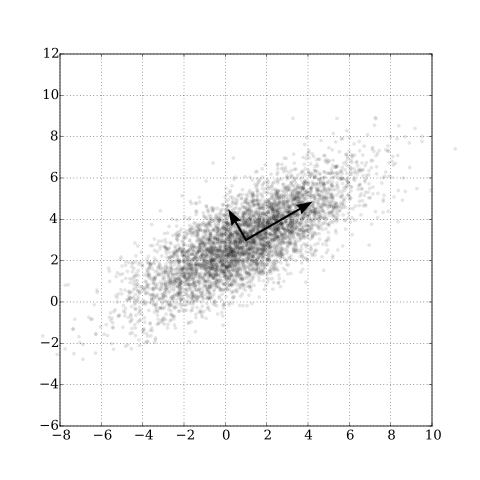
\includegraphics[width=0.5\textwidth]{GaussianScatterPCA.png}
        \caption{Datos con distribución Gaussiana y las dos primeras componentes PCA.}
        \label{fig:pca1}
    \end{figure}    
   
    Por ejemplo, la Figura~\ref{fig:pca1} representa un conjunto de datos de dos dimensiones con distribución Gaussiana. La flecha más grande representa la dirección de la primera componente principal de los datos. Se puede verificar a simple vista que esta es la dirección con mayor variabilidad en los datos. Si trazamos una línea imaginaria a lo largo de esa flecha (como la línea verde) y proyectamos en ella los datos, tendremos la proyección con mayor variabilidad. 
    
    La dirección de segunda componente está representada por la otra flecha. Al proyectar los datos en la línea imaginaria azul, podemos imaginar que el espectro de variabilidad es inferior al la primera.
   
    La proyección de un punto a una línea es muy sencilla: basta con buscar el punto más cercano en esa línea. Los puntos azules en la Figura~\ref{fig:pca_projection} representan la proyección de los puntos originales en la línea.

    \begin{figure}[h]
        \centering
        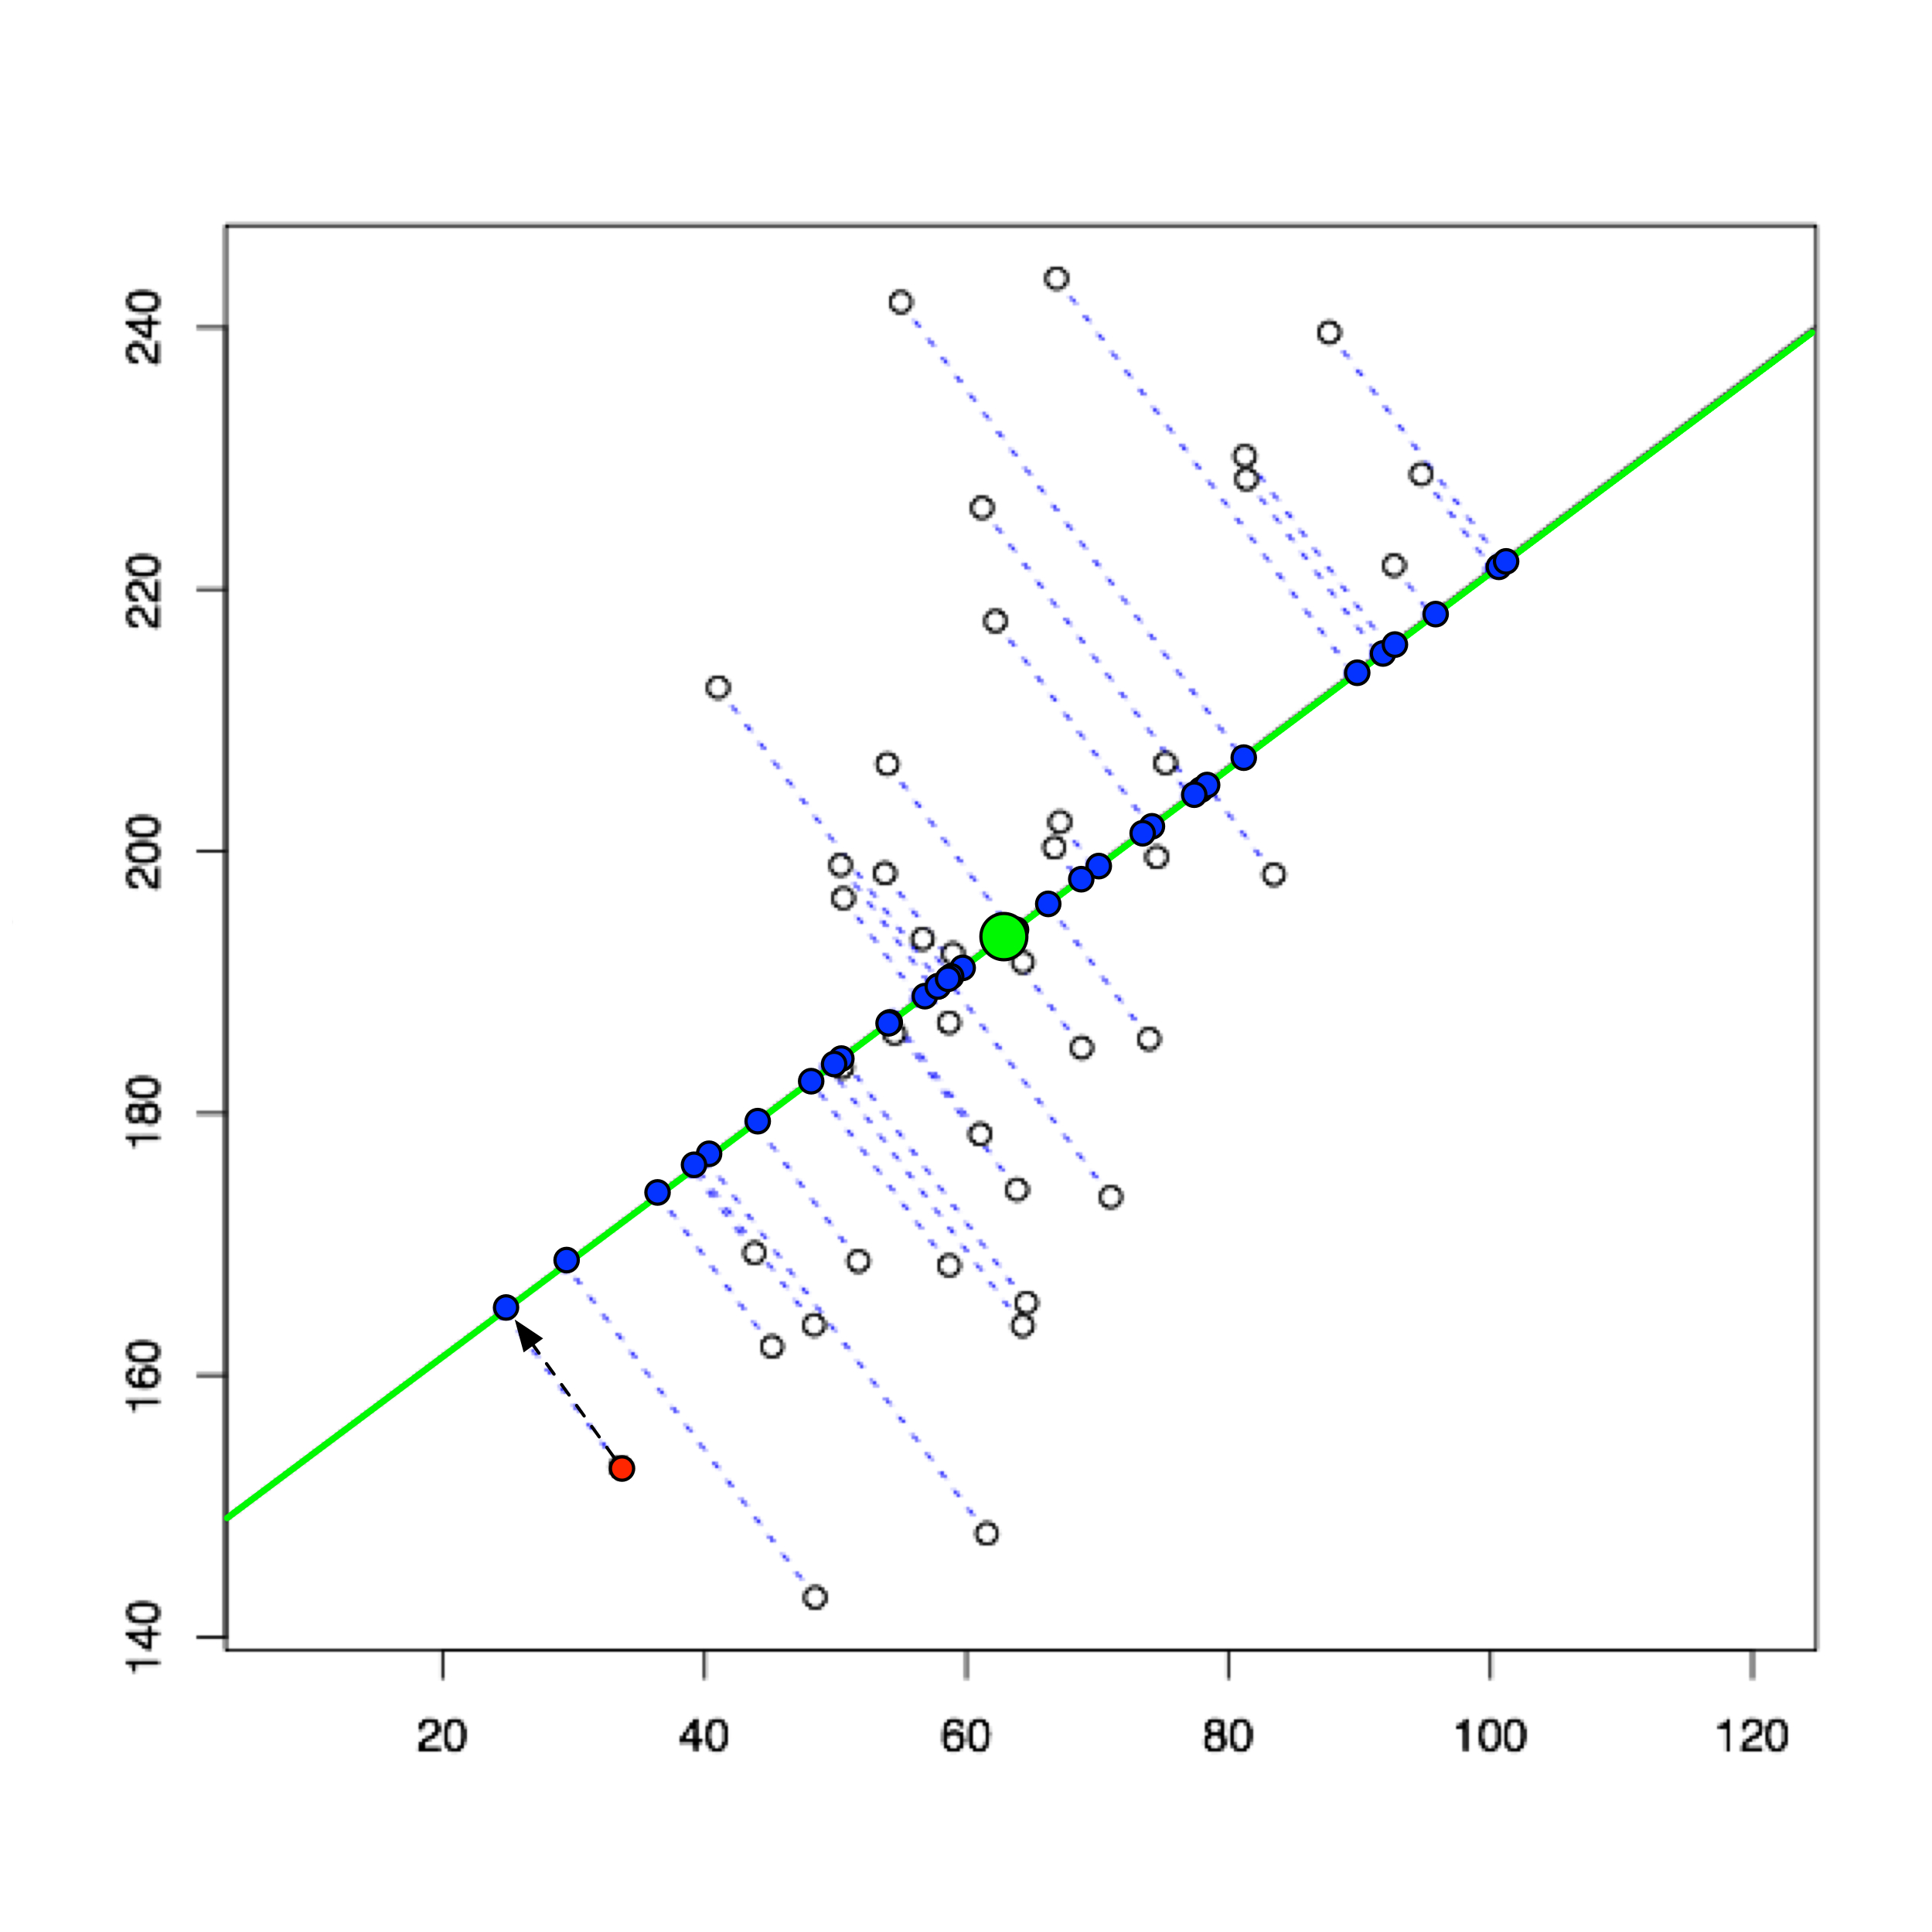
\includegraphics[width=0.5\textwidth]{ProjectionPCA.jpg}
        \caption{Proyección de puntos a una línea.}
        \label{fig:pca_projection}
    \end{figure}    
    
   En términos matemáticos, PCA es una transformación lineal ortogonal. Consideremos la matriz \(X\), constituida por \(n\) líneas de observaciones y \(m\) características. El objetivo es proyectar los datos a un espacio con dimensionalidad \(d < m\), de forma que se maximice la varianza de los datos proyectados. La transformación de PCA se define por la ecuación:
   \begin{equation}
   Y = X \cdot w
   \end{equation}
   
   Que se interpreta de la siguiente forma: una matriz \(m \times k\) de pesos ({\em loadings}) \(w\) transforma la matriz \(n \times m\) \(X\) en la matriz \(n \times k\) de componentes principales ({\em scores}) \(Y\).

   Para obtener la primera componente, el primer vector de {\em loadings} \(w\) debe maximizar la varianza. Siguiendo el razonamiento del libro \textit{Pattern Recognition and Machine Learning} \cite{bishop}, consideremos el vector \(w_{1}\), que, por conveniencia (y sin pérdida de generalización) debe ser un vector unitario de modo que \(w_{1}^{T}w_{1}=1\). Cada punto de X, \(x_{i}\), es proyectado para el escalar \(w_{1}^{T}x_{i}\). La media de los datos proyectados es \(w_{1}^{T} \overline{x}\), donde \(\overline{x}\) es la media dada por:
   \begin{equation}
   \overline{x} = \frac{1}{n}\sum_{i=1}^{n}x_{i}
   \end{equation}
   
   Y la varianza de los datos proyectados:
   \begin{equation}
   \frac{1}{n}\sum_{i=1}^{n}x_{i}\big\{w_{1}^{T}\cdot x_{i}-w_{1}^{T}\cdot \overline{x}\big\} = w_{1}^{T}\cdot S\cdot w_{1}
   \end{equation}
   
   Donde \(S\) es la matriz de varianzas-covarianzas definida por:
   \begin{equation}
   S=\frac{1}{n}\sum_{i=1}^{n}(x_{i}-\overline{x})\cdot (x_{i}-\overline{x})^{T}
   \end{equation}
   
   Ahora maximizamos la varianza de los datos proyectados \(w_{1}^{T}\cdot S\cdot w_{1}\) con respecto a \(w_{1}\). Hay que restringir la maximización para prevenir que tienda para infinito. La restricción viene de la normalización \(w_{1}^{T}w_{1}=1\). Para forzar la restricción introducimos un multiplicador de Lagrange \(\lambda_{1}\):
   \begin{equation}
   w_{1}^{T}\cdot S\cdot w_{1} + \lambda_{1} (1 - w_{1}^{T}\cdot w_{1})
   \end{equation}
   
   Que tiene un punto estacionario cuando:
   \begin{equation}
   S\cdot w_{1} = \lambda_{1} \cdot w_{1}
   \end{equation}
   
   Esto define que \(w_{1}\) es un vector propio de \(S\). Si multiplicamos las parte izquierda por \(w_{1}^{T}\), teniendo en cuenta que \(w_{1}^{T}w_{1}=1\), vemos que la varianza es dada por:
   \begin{equation}
   w_{1}^{T}\cdot S\cdot w_{1} = \lambda_{1} 
   \end{equation}
   
   Así que la varianza será máxima cuando se defina \(w_{1}\) igual al vector propio con el máximo valor propio \(\lambda_{1}\).
   
    \subsection{Singular Value Decomposition}
    PCA está muy relacionado con una técnica matemática llamada {\em Singular Value Decomposition} (SVD), tanto que muchas veces los nombres se usan intercambiados. De hecho, el algoritmo de PCA de {\tt scikit-learn} usa la descomposición SVD de {\tt numpy}. SVD es un método más general de entender el cambio de base.
    
    La representación de la descomposición en valores singulares es:
    \begin{equation}
    X = U \Sigma W^{T}
    \end{equation}
    
    Donde:
    \begin{itemize}
    \item \(U\) es una matriz \(n \times n\), en que las columnas son vectores unitarios ortogonales de tamaño \(n\).
    \item \(\Sigma\) es una matriz diagonal \(n \times m\) de números positivos \(\sigma_{i}\), llamados valores singulares de \(X\).
    \item \(W\) es una matriz \(m \times m\), cuyas columnas son vectores unitarios ortogonales de tamaño \(p\).
    \end{itemize}
    
    La ecuación 4.2 indica que una matriz \(X\) puede ser convertida en una matriz ortogonal, una matriz diagonal y otra matriz ortogonal. O, dicho de otra forma, corresponde a una rotación, un estiramiento y otra rotación.
    
    \subsection{El método NIPALS}
    SVD es el método general para cálculo de PCA. Pero si lo aplicamos a un {\em dataset} multidimensional muy grande puede tener problemas, porque calcula todas las componentes de una vez (calcula toda la matriz de varianzas-covarianzas de \(X\)). Esto implica un gran consumo de memoria y CPU. NIPALS significa {\em Non-linear Iterative Partial Least Squares} y es un algoritmo iterativo que solo calcula las primeras componentes principales.
    
    Para cada componente, el algoritmo NIPALS itera hasta que el {\em score} \(y_{1}\) tenga convergencia. Antes de la iteración, se atribuye un valor aleatorio al {\em score} \(y_{1}\). La convergencia se detecta cuando la variación del {\em score} \(y_{1}\) respecto a la iteración anterior es muy pequeña. 
    
     En cada iteración, para encontrar el {\em loading} \(w_{1}\) se proyecta \(X\) hacía \(y_{1}\) - regresión del {\em score} respecto a cada columna de \(X\) - y se guarda el coeficiente de regresión en el {\em loading}. Luego se proyecta \(X\) hacía \(w_{1}\) para encontrar el {\em score} \(y_{1}\) - regresión del {\em loading} respecto a cada línea de \(X\) - y se guarda el coeficiente de regresión en el {\em score}. 
    
    Una vez convergido, para calcular la siguiente componente se resta el producto \(y_{1} \cdot w_{1}\) a \(X\). Esto corresponde a restar a \(X\) la parte de los datos explicada por \(y_{1}\) y \(w_{1}\).
    
    TODO: Hotelling T2?
    
%    El nuevo espacio está constituido por variables independientes y ortogonales. Para cada componente, se calculan valores aleatorios con distribución normal. Estos son los scores de las componentes de los nuevos datos. Al proyectar la nueva matriz de componentes de vuelta al espacio original, se obtienen datos simulados para todas las características. Si la validación de esta técnica demuestra que es correcta, se puede usar para la simulación de nuevos datos. La validación de los datos generados pasa por la aplicación de estadísticos de comparación de las muestras originales y las nuevas. La técnica utilizada es el test de Hotelling T-squared, que prueba la similitud de las poblaciones. Los resultados demuestran que es viable usar esta técnica de simulación de datos.

    \section{Series temporales - ARIMA}
    Las series temporales surgen frecuentemente en la monitorización de procesos industriales. Cada observación de un sensor tiene una marca temporal asociada. El conjunto de las observaciones ordenadas de forma cronológica se denomina serie temporal. En este capítulo se demostrará el importante valor que tiene esa marca temporal en el análisis de las señales. 
    
    El análisis de series temporales asienta en la suposición de que los datos tomados en determinados puntos en el tiempo tienen una estructura interna (correlación, tendencia o variación estacional) que hay que tener en cuenta. El objetivo del análisis de series temporales es extrapolar datos futuros a través de los datos pasados. 
    
    ARIMA significa ({\em Autoregressive Integrated Moving Average}) y, junto con ({\em Exponential Smoothing}), es uno de los métodos más populares de análisis de series temporales. ARIMA incorpora formalmente la dependencia entre observaciones sucesivas en el modelo, mientras {\em Exponential Smoothing}) no lo hace de forma tan eficiente.
    
    La componente AR ({\em Autoregressive} - auto-regresiva) del modelo ARIMA se refiere al uso de observaciones anteriores en una ecuación regresiva para predecir valores futuros. A esta componente se asocia un parámetro \(p\), que corresponde al numero de puntos anteriores a incluir en el modelo. La componente MA ({\em Moving Average} - media móvil) representa el error del modelo como combinación de términos de error anteriores. El parámetro asociado es \(q\) y corresponde al numero de términos de error anteriores a usar. La componente I ({\em Integrated}) indica la diferenciación de los datos, que corresponde a calcular la diferencia entre los valores y sus antecesores. El parámetro \(d\) es el numero de diferenciaciones a aplicar en el modelo. De esta forma, los modelos ARIMA son generalmente definidos por \(ARIMA(p, d, q)\).
    
    Es importante resaltar que el modelo \(ARIMA(p, d, q)\) asume que la serie no tiene variación estacional y tendencia. Potencialmente es necesario eliminar esas características antes de crear el modelo. Esto nos lleva al concepto de {\em stationarity} (estacionaridad).
    
    \subsection{Estacionaridad}
    Las series temporales son diferentes de un problema de regresión normal porque son dependientes del tiempo. Así que el supuesto básico de la regresión lineal de que las observaciones son independientes no se verifica en este caso. Para poder aplicar el modelo ARIMA es necesario que la serie sea estacionaria. Una serie es estacionaria cuando la media y varianza, si existen, no cambian en función del tiempo. Como ARIMA usa los periodos anteriores para modelar el comportamiento de la serie, es importante que esta sea estable para tener más acierto. Muchas veces la estacionaridad se puede detectar visualmente, como se presenta en los ejemplos siguientes.
    
    La Figura~\ref{fig:stationary} es un ejemplo de una serie estacionaria, donde los valores oscilan con una varianza constante alrededor de una media de aproximadamente \(69.0\). 
    
    \begin{figure}[h]
        \centering
        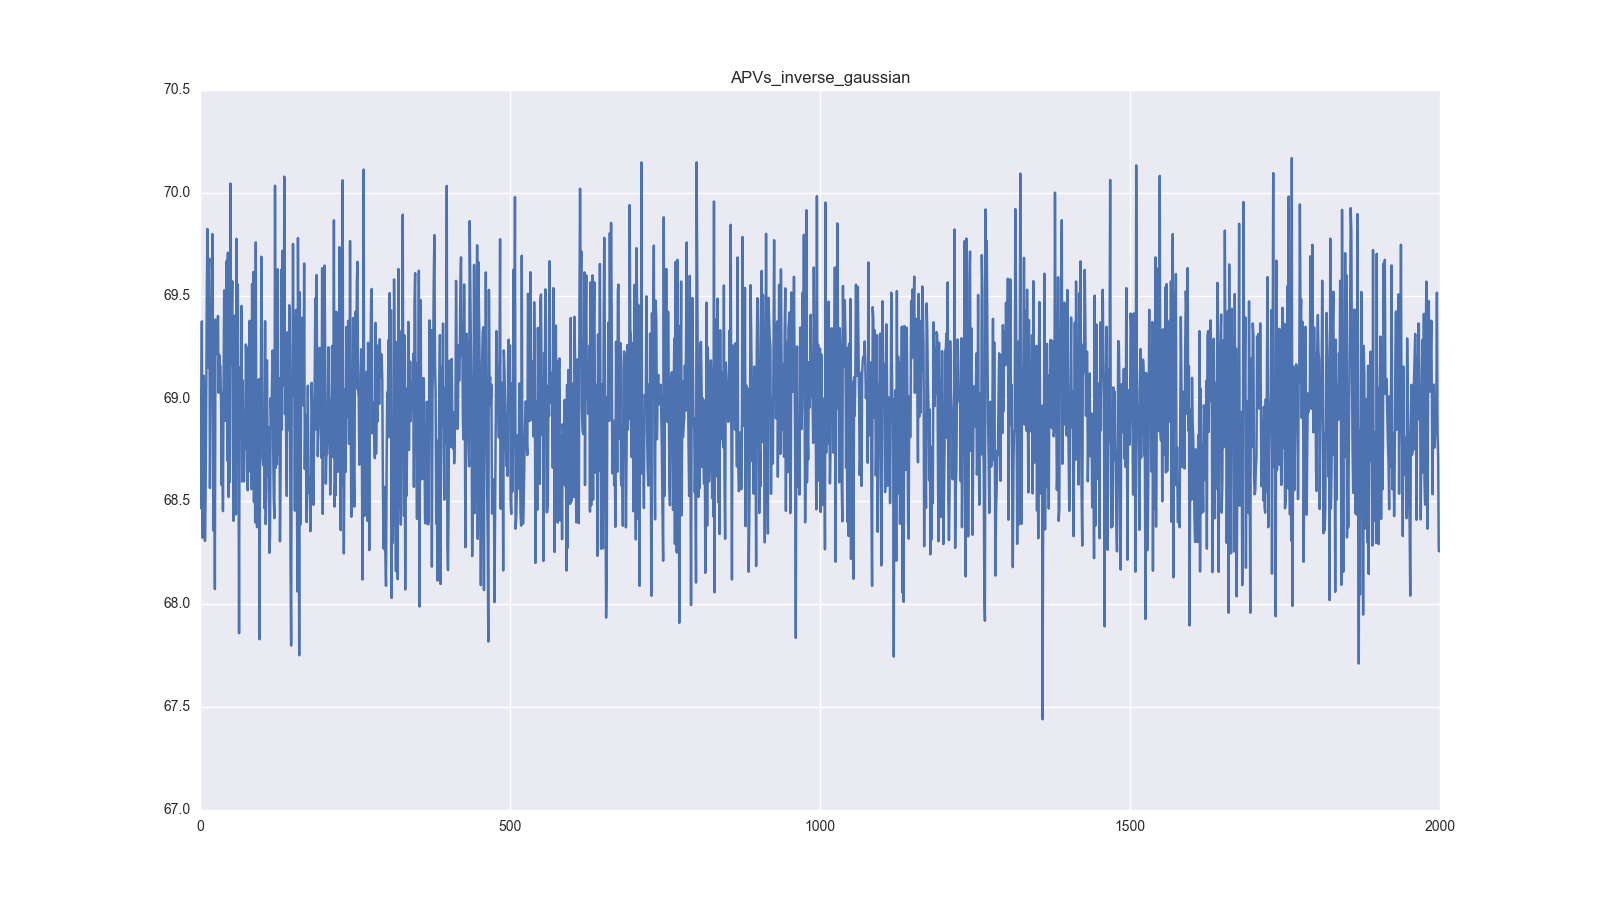
\includegraphics[width=0.7\textwidth]{APVs_inverse_gaussian.png}
        \caption{Ejemplo de serie estacionaria.}
        \label{fig:stationary}
    \end{figure}

    La Figura~\ref{fig:non_stationary}, sin embargo, no presenta señales de media y varianza constantes. De hecho se detecta una ligera tendencia decreciente, lo que la hace no estacionaria. 
    
    \begin{figure}[h]
        \centering
        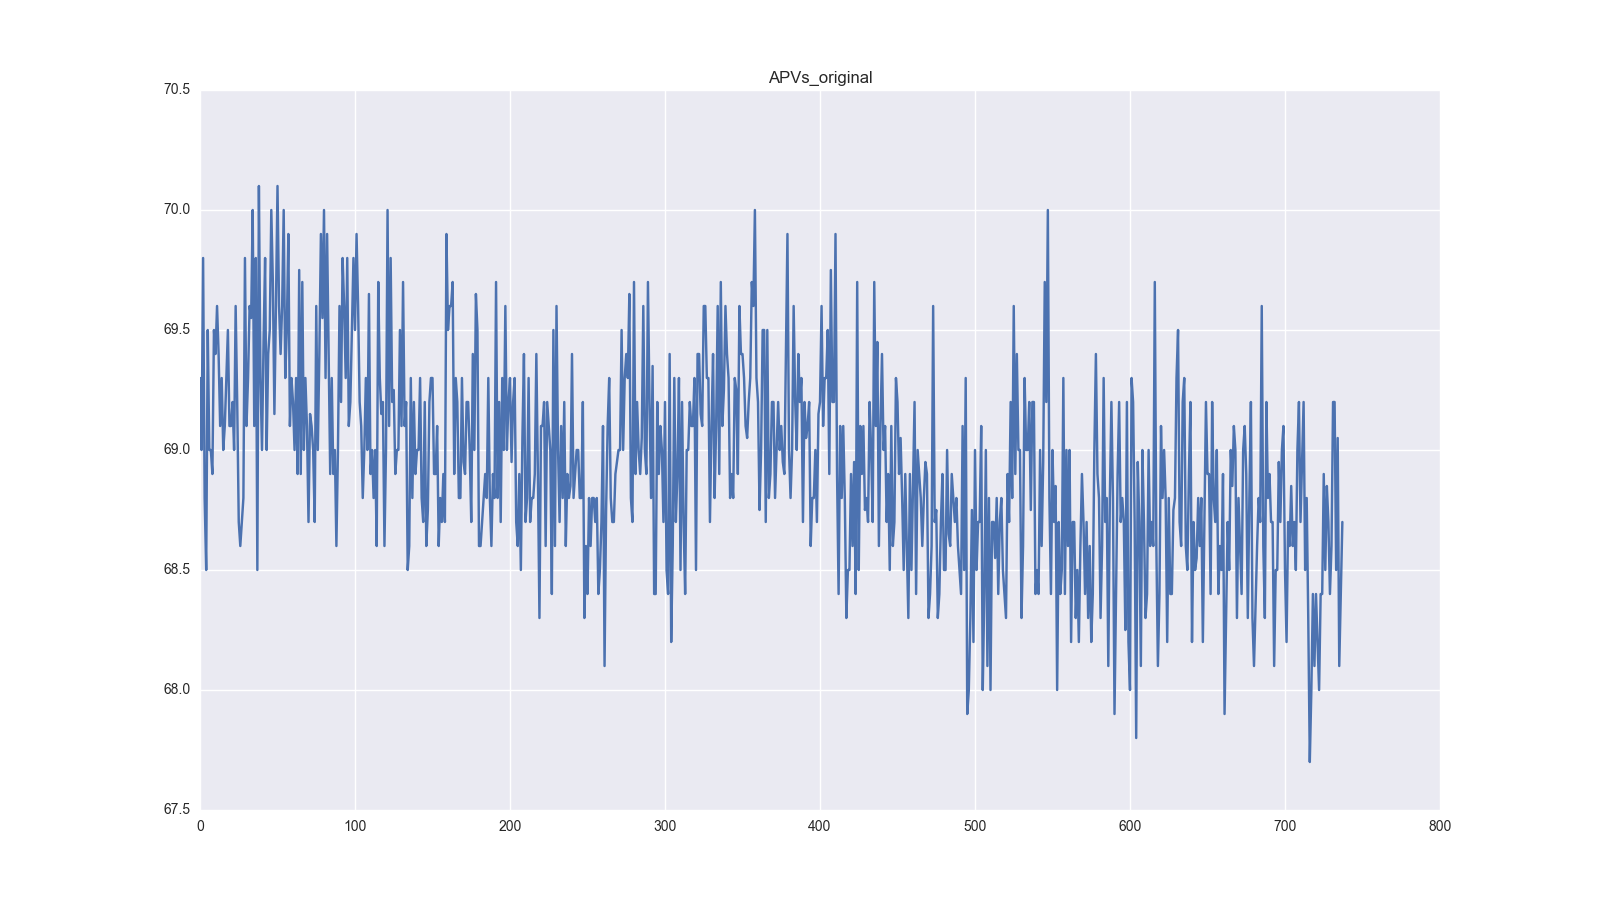
\includegraphics[width=0.7\textwidth]{APVs_original.png}
        \caption{Ejemplo de serie no estacionaria.}
        \label{fig:non_stationary}
    \end{figure}
    
    Otra propiedad importante para que ARIMA sea efectivo es que la serie tenga periodos fijos. Cada observación debe ser dada a una frecuencia constante. Una vez los puntos sean equidistantes entre si, la variable tiempo, o índice, ya no necesita existir explicitamente. Muchas veces se usa el tiempo para la representación gráfica, sin embargo esa variable no se usa en el modelo en si. En los gráficos anteriores no se usa la marca de tiempo en el eje \(x\), simplemente un índice numerico. 
    
    Hay casos donde la estacionaridad es más difícil de determinar a simple vista. Además el análisis necesita una prueba formal de la estacionaridad. Para eso se usa el test estadístico de Dickey-Fuller, conocido por {\em augmented Dickey-Fuller test} (ADF). La hipótesis nula asume que la serie es no estacionaria. Valores altos del p-valor indican que el test no rechaza la hipótesis nula y, por lo tanto, la serie es no estacionaria. Por otro lado, valores bajos de p-valor indican que la serie es estacionaria. En general, tomando el 5\% de confianza, si el p-valor es mayor que 0.05 la serie es no estacionaria. Se demuestra en el ejemplo siguiente.
    
    %ADF procedure tests whether the change in Y can be explained by lagged value and a linear trend. If contribution of the lagged value to the change in Y is non-significant and there is a presence of a trend component, the series is non-stationary and null hypothesis will not be rejected.
    
    \begin{figure}[h]
        \centering
        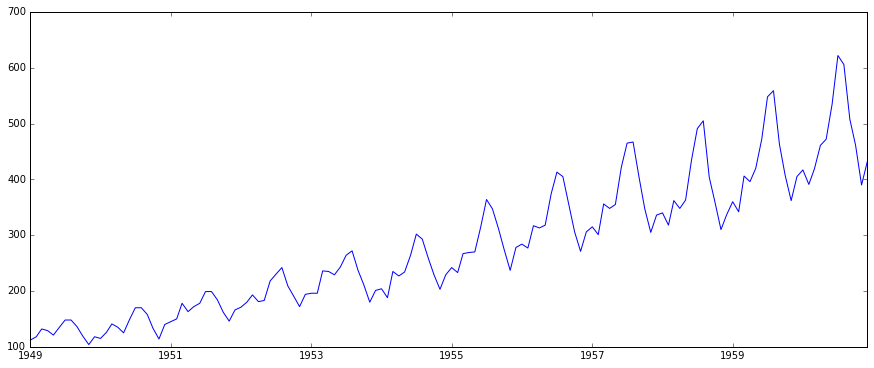
\includegraphics[width=0.7\textwidth]{time_serie_1.png}
        \caption{Ejemplo de serie para aplicar el test de Dickey-Fuller.}
        \label{fig:time_serie_1}
    \end{figure}
    
    La serie de la Figura~\ref{fig:time_serie_1} tiene una tendencia creciente, por lo que no debería ser estacionaria. Apliquemos el test de Dickey-Fuller, presente en módulo {\tt statsmodels} de Python:
    
    \lstset{style=python}
    \begin{lstlisting}[caption=Test de Dickey-Fuller de {\tt statsmodels} de Python., label={lst:adf_test_1}]
from statsmodels.tsa.stattools import adfuller
dftest = adfuller(ts)
print('Test Statistic', dftest[0])
print('p-value', dftest[1])
print('Confidence levels', dftest[4])  
    \end{lstlisting}
    
    \lstset{style=python}
    \begin{lstlisting}[caption=Resultados del test de Dickey-Fuller de {\tt statsmodels} de Python., label={lst:adf_res_1}]
Test Statistic 0.815368879206
p-value 0.991880243438
Confidence levels {'1%': -3.4816817173418295, '5%': -2.8840418343195267, '10%': -2.5787700591715979}
    \end{lstlisting}
    
    Los resultados del Listing~\ref{lst:adf_test_1} demuestran que la hipótesis nula no puede ser descartada, una vez que {\em p-value} es cercano a 1. El resultado del estadístico lo confirma también: para que se descarte la hipótesis nula, el valor del estadístico debe ser inferior a alguno de los valores de los intervalos de confianza.
    
    La serie tendrá que ser transformada hasta ser estacionaria. Una de las técnicas más comunes para conseguirlo es la diferenciación, que consiste en calcular las diferencias entre observaciones consecutivas. La diferenciación ayuda a estabilizar la media de la serie, eliminando la tendencia y la estacionalidad. El primer nivel de diferenciación de la serie \(y\) se define por:
    
    \begin{equation}
    y_{t}-y_{t-1}
    \end{equation}
    
    Siendo \(t\) un determinado punto en el tiempo. Se pueden aplicar más niveles de diferenciación, pero con un solo nivel suele ser suficiente.
    
    Aplicando diferenciación a la serie anterior obtenemos la serie transformada representada en la Figura~\ref{fig:ts_diff} y respectivos resultados en Listing~\ref{lst:adf_test_2}.
    
    \begin{figure}[h]
        \centering
        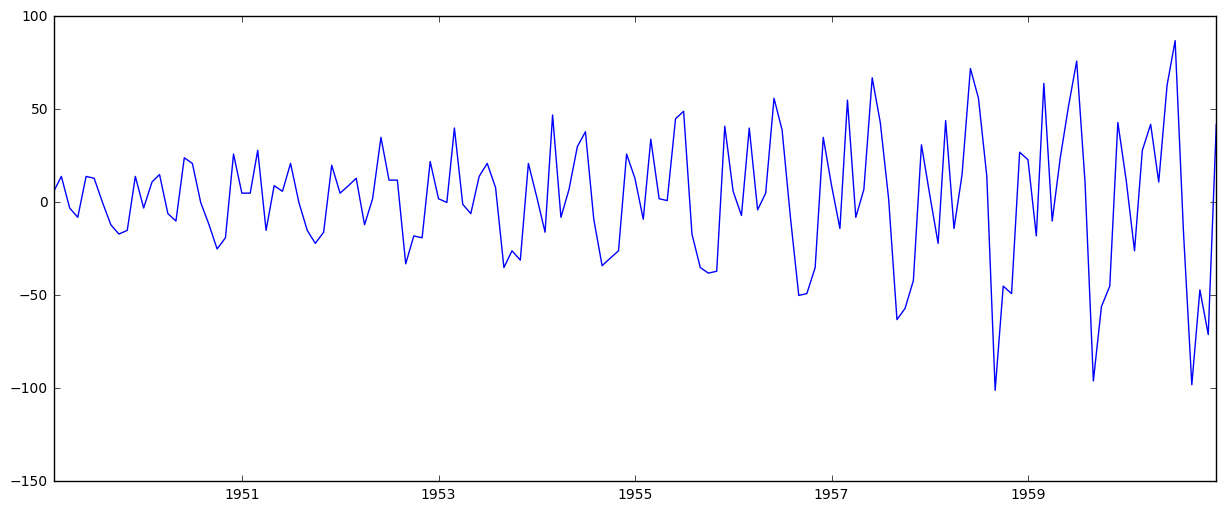
\includegraphics[width=0.7\textwidth]{ts_diff.png}
        \caption{Ejemplo de serie con diferenciación.}
        \label{fig:ts_diff}
    \end{figure}
    
    \begin{lstlisting}[caption=Resultados del test de Dickey-Fuller de {\tt statsmodels} de Python., label={lst:adf_test_2}]
Test Statistic -2.82926682417
p-value 0.0542132902838
Confidence levels {'1%': -3.4816817173418295, '5%': -2.8840418343195267, '10%': -2.5787700591715979}
    \end{lstlisting}
    
    El test de Dickey-Fuller demuestra que el p-valor ha bajado considerablemente, para valores casi inferiores a \(0.05\), por lo que podemos decir con un 95\% de confianza que la serie es estacionaria ahora. El análisis visual también permite verificar que la tendencia se ha eliminado.
    
    \subsection{Parámetros del modelo y predicción}
    
    Como mencionado anteriormente, el modelo ARIMA es una ecuación lineal que depende de los parámetros \(p, d, q\), correspondientes a las partes autoregresiva (AR), integración (I) y de medias móviles (MA) del modelo, respectivamente. 
    
    El paso de diferenciación es aplicado internamente por el modelo, a través del parámetro \(d\), que corresponde a la parte I ({\em Integrated}) de ARIMA. No hace falta pasar los datos diferenciados al modelo. Para la determinación de los parámetros \(p\) y \(q\) óptimos se usan formalmente los gráficos de correlación ACF ({\em Auto-Correlation Function}) y PACF ({\em Partial Auto-Correlation Function}). Estos gráficos se han usado en fases iniciales de este estudio, pero salen del ámbito de investigación. 
    
    Otra solución es la minimización del error, o valor residual, de la predición. La diferencia entre la observación \(y_{t}\) y el valor obtenido a través del ajuste del modelo a los datos (o valor ajustado \(y'_{t}\)) se llama valor residual, y es definido por:
    
    \begin{equation}
    e_{t} = y_{t} - y'_{t}
    \end{equation}
    
    A través de los residuales se puede calcular el {\em root mean squared error} (RMSE). El modelo con menor RMSE es el mejor. Así que la solución consiste en iterar, probando todas las combinaciones de los parámetros \((p,d,q)\) de ARIMA, para obtener el modelo con menor RMSE. Se ejemplifica el proceso a continuación.
    
    Se ha comprobado antes que la serie necesita un nivel de diferenciación para ser estacionaria: \(d=1\). La componente I de ARIMA será tendrá, así, valor \(1\). 
    
    Empezamos la iteración con un nivel para la componente auto-regresiva: \(p=1\), que corresponde a \(AR(1)\). El resultado del ajuste del modelo se puede ver en la Figura~\ref{fig:iterative_arima_ar_1}. La línea azul representa los datos de la serie diferenciada y la línea roja es el ajuste del modelo a esos datos. El RMSE es de \(\approx32.04\). 
    
    \begin{figure}[h]
        \centering
        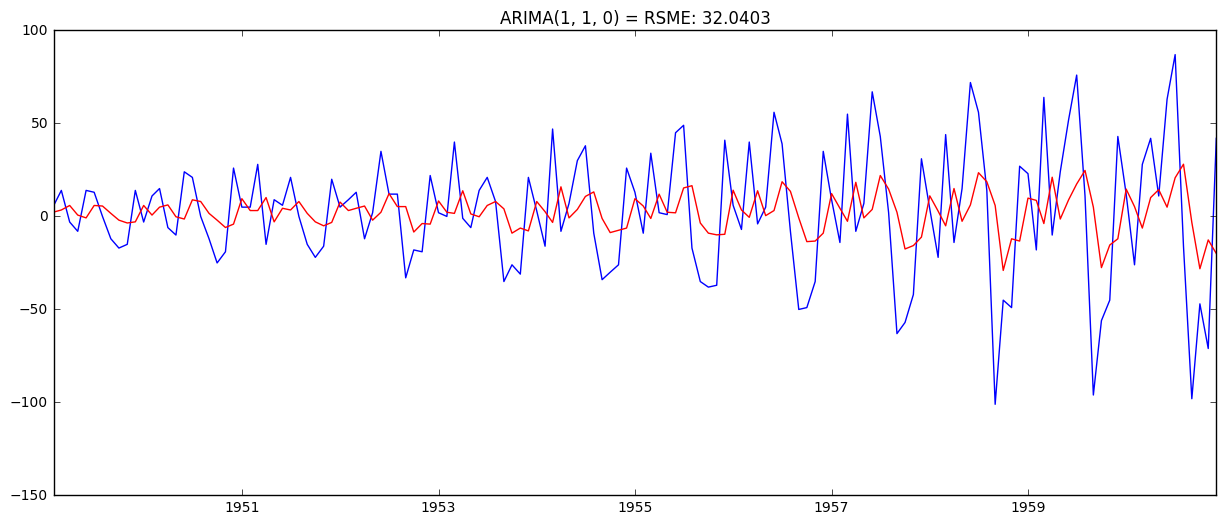
\includegraphics[width=0.7\textwidth]{arima_110.png}
        \caption{ARIMA iterativo: AR(1).}
        \label{fig:iterative_arima_ar_1}
    \end{figure}
    
    Pasamos a probar la componente de média móvil: \(q=1\), o \(MA(1)\). El RMSE ha bajado un poco, ahora es \(\approx31.52\) (Figura~\ref{fig:iterative_arima_ma_1}).
    
    \begin{figure}[h]
        \centering
        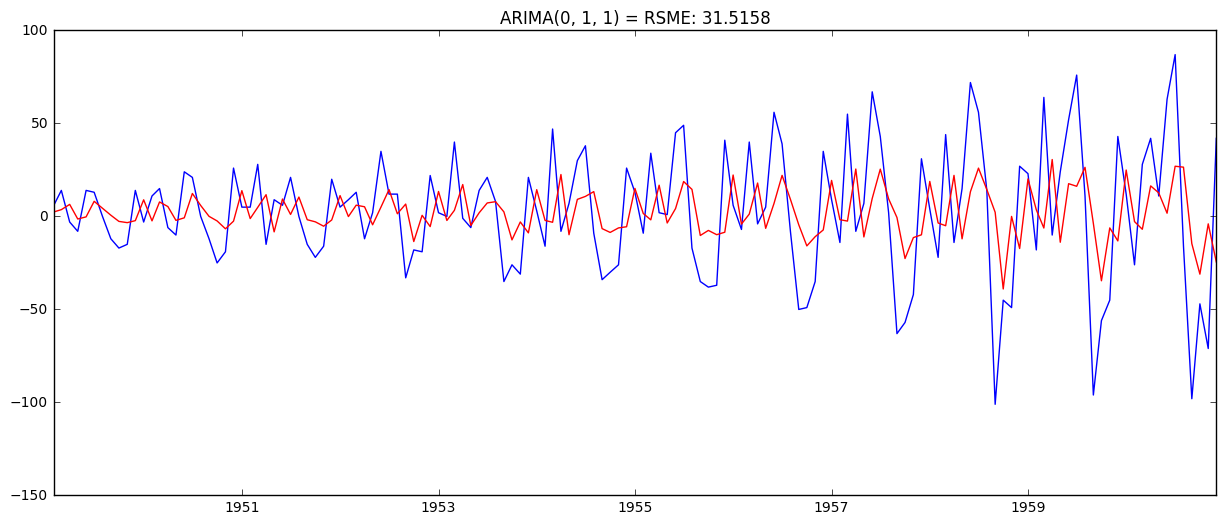
\includegraphics[width=0.7\textwidth]{arima_011.png}
        \caption{ARIMA iterativo: MA(1).}
        \label{fig:iterative_arima_ma_1}
    \end{figure}
    
    Combinando los dos modelos anteriores es cuando tenemos realmente un modelo ARIMA completo, con las tres componentes: \(ARIMA(p, d, q)=ARIMA(1, 1, 1)\). Se puede verificar que el RMSE ha bajado mínimamente respecto al modelo anterior (Figura~\ref{fig:iterative_arima_arma_1}).
    
    \begin{figure}[h]
        \centering
        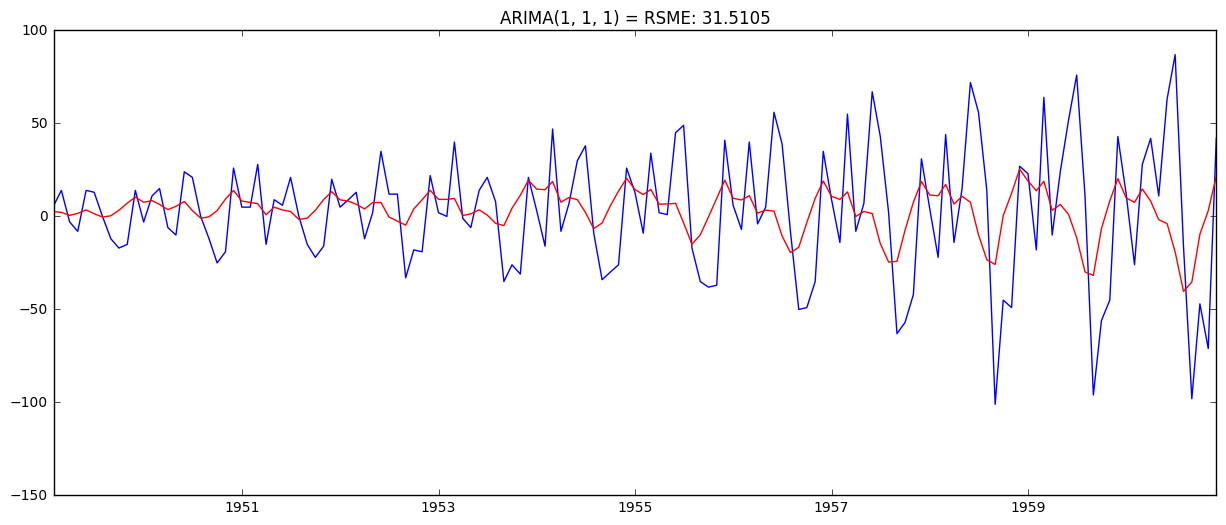
\includegraphics[width=0.7\textwidth]{arima_111.png}
        \caption{ARIMA iterativo: AR(1) y MA(1).}
        \label{fig:iterative_arima_arma_1}
    \end{figure}
        
    Obviando algunas iteraciones intermedias, pasamos al modelo con dos niveles de \(AR\) y de \(MA\): \(ARIMA(p, d, q)=ARIMA(2, 1, 2)\). El RMSE obtenido es de \(\approx25.06\), que corresponde al menor valor. Si paramos la iteración, este sería el modelo con mejor ajuste. En la Figura~\ref{fig:iterative_arima_arma_2} podemos verificar ese ajuste visualmente: la línea roja se ajusta mejor a los datos que en los gráficos anteriores.
  
    \begin{figure}[h]
        \centering
        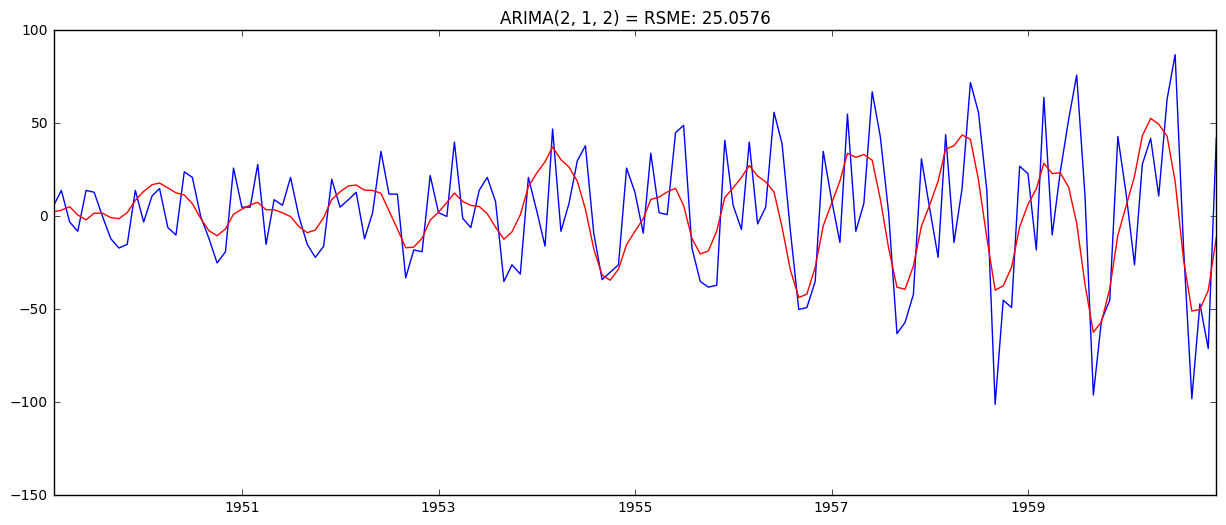
\includegraphics[width=0.7\textwidth]{arima_212.png}
        \caption{ARIMA iterativo: AR(2) y MA(2).}
        \label{fig:iterative_arima_arma_2}
    \end{figure}
    
    estadísticas, incluyendo modelos de series temporales. Particularmente útil es la funcionalidad de generar gráficas de predicción automáticamente, sin necesidad de volver los datos a la escala original (sin diferenciación), usando {\tt plot\_predict}. 

    Una vez ajustado el modelo a los datos, se pueden hacer predicciones futuras. Se define el periodo de predicción y el modelo aprendido generará esos pronósticos. La Figura~\ref{fig:forecast} da un ejemplo de los resultados que se pueden obtener. 

    \begin{figure}[h]
        \centering
        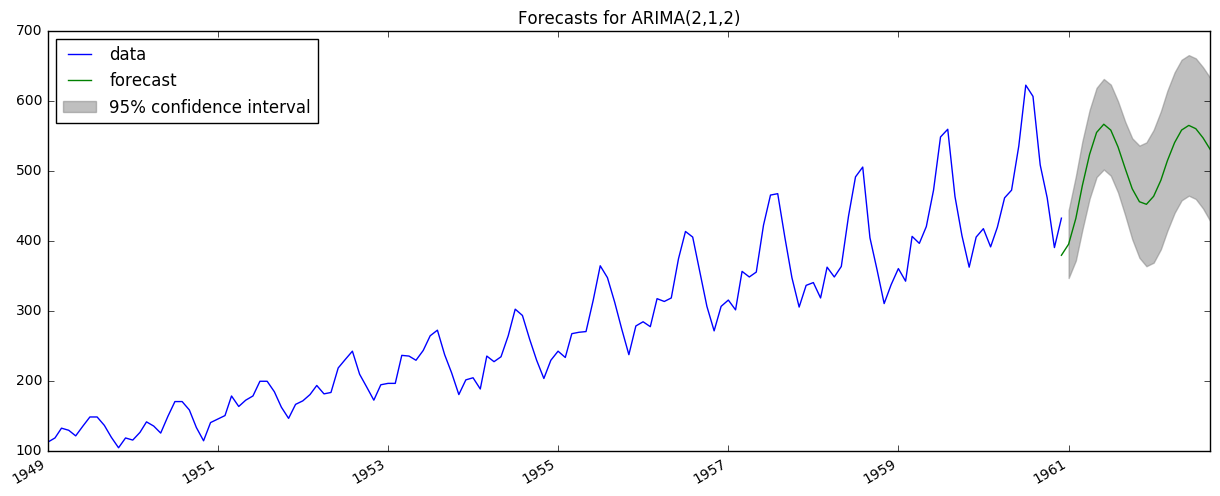
\includegraphics[width=0.7\textwidth]{forecast.png}
        \caption{Predicciones del modelo ARIMA(2, 1, 2).}
        \label{fig:forecast}
    \end{figure}

    La línea azul de la Figura~\ref{fig:forecast} representa los datos, ahora sin diferenciación. La línea verde representa la predicción después del final de la serie (llamada predicción {\em out-of-sample}). El área sombreada representa el intervalo de confianza de 5\% de la predicción. Se puede comprobar visualmente que la predicción sigue aproximadamente la tendencia de la serie. Predicciones con mayor horizonte futuro tendrán mayor incertidumbre, una vez que el modelo hará regresión de los valores futuros con los valores predichos.

    El modulo {\tt statsmodels} de Python tiene un conjunto de herramientas estadísticas, incluyendo modelos de series temporales. Particularmente útil es la funcionalidad de generar gráficas de predicción automáticamente, sin necesidad de volver los datos a la escala original (sin diferenciación en este caso), usando {\tt plot\_predict}. El Listing~\ref{lst:forecast} es el código que genera el gráfico de la Figura~\ref{fig:forecast}. El periodo de predicción está aquí definido en los parámetros {\tt start} y {\tt end}, en un total de 20 nuevos puntos desde el final de la serie ({\tt len(ts)}).

    \lstset{style=python}
    \begin{lstlisting}[float, caption={\tt plot\_predict} de {\tt statsmodels} de Python., label={lst:forecast}]
from statsmodels.tsa.arima_model import ARIMA
model = ARIMA(ts, order=(2, 1, 2))
results = model.fit(disp=-1)
fig, ax = plt.subplots()
plt.plot(ts)
fig = results.plot_predict(start=len(ts)-1, end=len(ts)+20, dynamic=True, ax=ax, plot_insample=False)
    \end{lstlisting}


% Experimentación y resultados
\chapter{Experimentación y resultados}
TODO

    % Dataset
    \section{Dataset}
    El dataset proporcionado es de reducida dimensión, tiene tan solo 5MB, por lo que la tarea de ingestión no es intensiva. Sin embargo, hay que tratar los datos en bruto antes de empezar a usarlos. El fichero de datos es de texto, así que hay que hacer determinadas conversiones para poder usar tipos más específicos, como sean fechas y números. El primer problema tiene que ver con los formatos de fecha, que no son correctos para el {\em locale} España en {\em Windows}, lo que exige una adaptación de los algoritmos de {\em parsing}, como se describe en el apartado 'Transformación'.
    
        \subsection{Estructura}
        Un breve análisis del {\em dataset} en un editor de texto muestra que tiene un formato de campos separados por espacios y tabulaciones. La cantidad de espacios es variable:
    
        \lstset{style=default}
        \lstset{
          showspaces = true
        }
        \begin{lstlisting}[caption=Ejemplo del {\em dataset}.]
        Tiempoinicio                    	APHu                            	APVs ...
        
        06-oct-2015 21:57:03 	44.6             	69.3 ...
        06-oct-2015 21:57:12 	45.1             	69.0 ...
        06-oct-2015 21:57:21 	44.8             	69.8 ...
        ...
        \end{lstlisting}
        
        \lstset{
          showspaces = false
        }
        La primera línea contiene un {\em header} (cabecera), con 15 nombres: 
        \begin{lstlisting}[caption={\em Header} del {\em dataset}.]
        Tiempoinicio APHu APVs ACPv ZSx ZUs H7x H1x H2x H6x H3x H4x H5x ACPx Svo
        \end{lstlisting}
        
        Se puede verificar también que hay una línea vacía después del {\em header}. El primer campo tiene un formato de fecha/hora y los demás campos tienen formato decimal.
    
        \subsection{Transformación}
        Para la ingestión y transformación de los datos se han usado librerías muy útiles y con muchas funcionalidades que facilitan bastante esas tareas: en los scripts Python se ha usado el paquete {\em Pandas} y en R la función {\em read.csv2} del paquete {\em utils}.
        
        Las 14 variables decimales no ofrecen problemas en la ingestión del {\em dataset}. Para asegurar el formato decimal, es conveniente definir el separador decimal como punto ('.'). Con eso es suficiente para un {em parsing} correcto.
        
        Las fechas son más complejas de procesar. El formato de mes da indicios de estar escrito en castellano: {\tt oct, dic, mar, abr, may, jun}. Sin embargo, en {\em Windows}, el {\em locale} España usa un punto ('.') como {\em standard} en la abreviación de mes, por ejemplo 'oct.'. Así que el {\em parsing} de fechas tiene que ser ajustado si el sistema operativo es {\em Windows}. La estrategia ha sido el uso de una expresión regular para añadir el punto ('.') necesario en las abreviaciones de meses, como se puede ver en los siguientes {\em snippets} Python y R:
        
        \lstset{style=python}
        \begin{lstlisting}[caption={\em Parsing} de fechas en Python.]
def parse_date(date_string):
    locale_date_string = re.sub("(.+-)(.+)(-.+)", "\\1\\2.\\3", date_string)
    return datetime.strptime(locale_date_string, "%d-%b-%Y %H:%M:%S")
        \end{lstlisting}
        
        \begin{lstlisting}[caption={\em Parsing} de fechas en R.]
data$Tiempoinicio <- sub("(\\d+-)(\\w+)(-\\d+\\s\\d+:\\d+:\\d+)", "\\1\\2.\\3", data$Tiempoinicio)
data$Tiempoinicio <- as.POSIXct(data$Tiempoinicio, format="%d-%b-%Y %H:%M:%S")
        \end{lstlisting}
        
        En este caso particular de las fechas, el problema no está en el {\em dataset} realmente. Los {\em standards} de fechas varian en cada sistema operativo. La idea de exponer este caso no es más que transmitir la necesidad de ajustar y normalizar los datos cuando provienen de sensores.
        
        El resultado final es un {\em dataset} estructurado con una marca temporal como índice y 14 características: {\em APHu, APVs, ACPv, ZSx, ZUs, H7x, H1x, H2x, H6x, H3x, H4x, H5x, ACPx} y {\em Svo}.
        
        \subsection{Distribución de los datos}
        
        Las mediciones de los sensores se distribuyen por varios días, no siempre consecutivos. Los días con mediciones son algunos 
        \begin{itemize}
        \item 6-9, 12 de octubre de 2015
        \item 14 de diciembre de 2015
        \item 7, 8, 11, 14 de marzo de 2016
        \item 6, 29 de abril de 2016
        \item 2, 26 de mayo de 2016
        \item 8, 17, 20 de junio de 2016
        \end{itemize}
        
        En cada día las muestras son dispares y en momentos distintos del día, probablemente por corresponder a distintas pruebas. Así, también las frecuencias de muestreo son variables - en algunos días parece indicar una frecuencia de 10 segundos pero hay otros donde son de 1 minuto.
    
    % PCA
    \section{PCA}
    A continuación se presentan las pruebas realizadas para el cálculo de las componentes principales (PCA) del {\em dataset} y respectiva inversión al espacio original. Los primeros análisis son informales, sobre todo con recurso a gráficos. Luego se formalizan estos resultados por medio de un test estadístico. El capítulo termina con una propuesta de simulación de datos, que, respaldada por el test estadístico, servirá de base para las fases siguientes.
    
    % NIPALS
    \subsection{PCA iterativo - NIPALS}
    Para {\em datasets} grandes, el algoritmo iterativo NIPALS ofrece mejor rendimiento, al determinar solamente el numero de componentes definido. SVD calcularía la matriz de varianzas-covarianzas para todos los componentes, lo que exigiría mucha memoria y CPU. Aunque en este caso el {\em dataset} es pequeño, usaremos el algoritmo iterativo NIPALS.
    
    Empezamos por analizar visualmente los datos de sensores para un día determinado. Observemos el comportamiento de la variable {\em APVs} para ese día, representado en la Figura~\ref{fig:APVs_original}. 
    
    \begin{figure}[h]
        \centering
        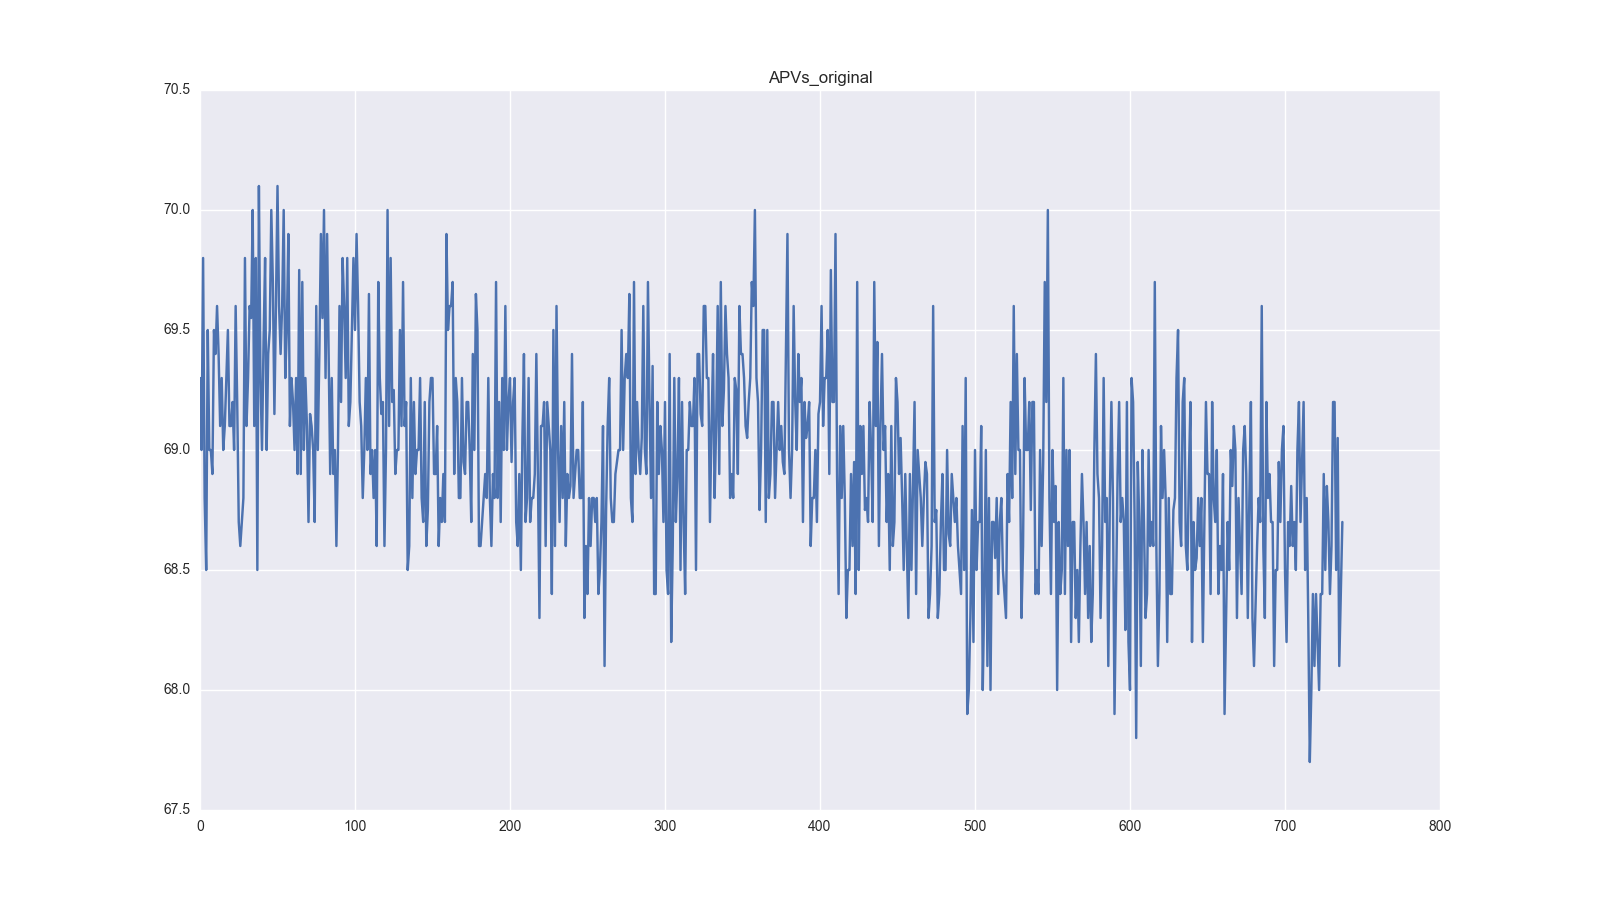
\includegraphics[width=0.7\textwidth]{APVs_original.png}
        \caption{Datos originales de la variable {\em APVs}.}
        \label{fig:APVs_original}
    \end{figure}
    
    Aplicamos el algoritmo iterativo NIPALS para calcular las 5 componentes principales, proyectando de esta forma el espacio original de 14 dimensiones (características) en un espacio más reducido de solamente 5 dimensiones. Al invertir este espacio de vuelta al espacio original se obtienen datos muy similares a los originales, como se puede comprobar informalmente en la Figura~\ref{fig:APVs_inverted_nipals}, que representa los datos invertidos para la variable {\em APVs}.
    
    Obviamente se podría usar la descomposición SVD para el cálculo de las componentes principales. Usando SVD de {\tt numpy} se obtienen los mismos resultados, que se pueden analizar informalmente en la Figura~\ref{fig:APVs_inverted_svd}. 
    
    \begin{figure}[H]
        \centering
        \begin{subfigure}[h]{0.49\textwidth}
            \centering
            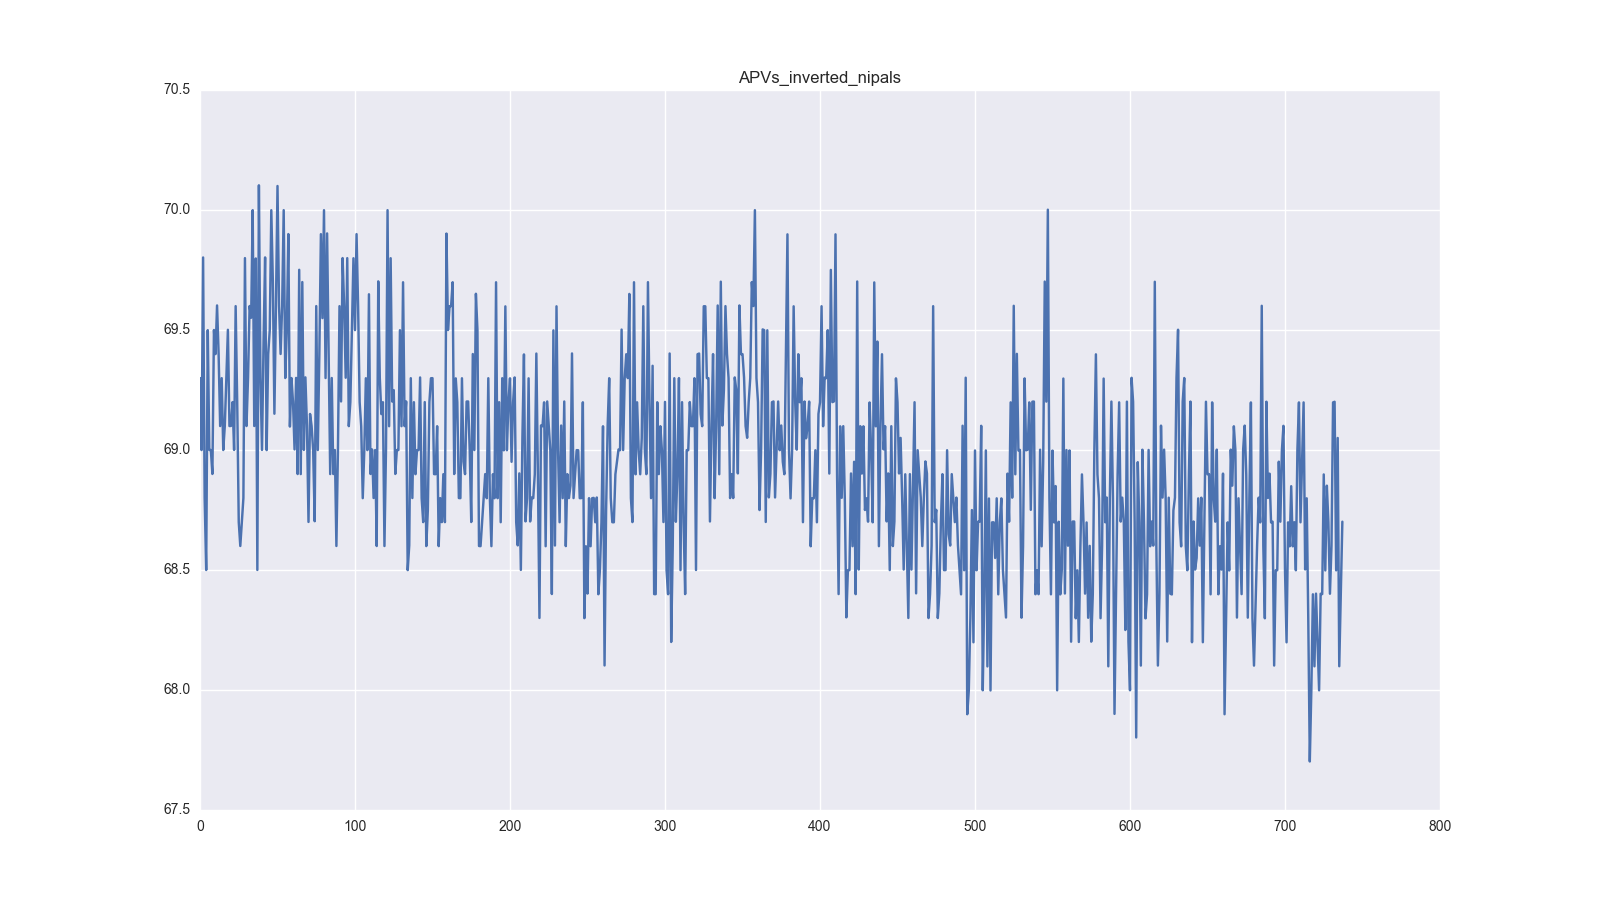
\includegraphics[width=\textwidth]{APVs_inverted_nipals.png}
            \caption{Inversión de NIPALS.}
            \label{fig:APVs_inverted_nipals}
        \end{subfigure}
        \begin{subfigure}[h]{0.49\textwidth}
            \centering
            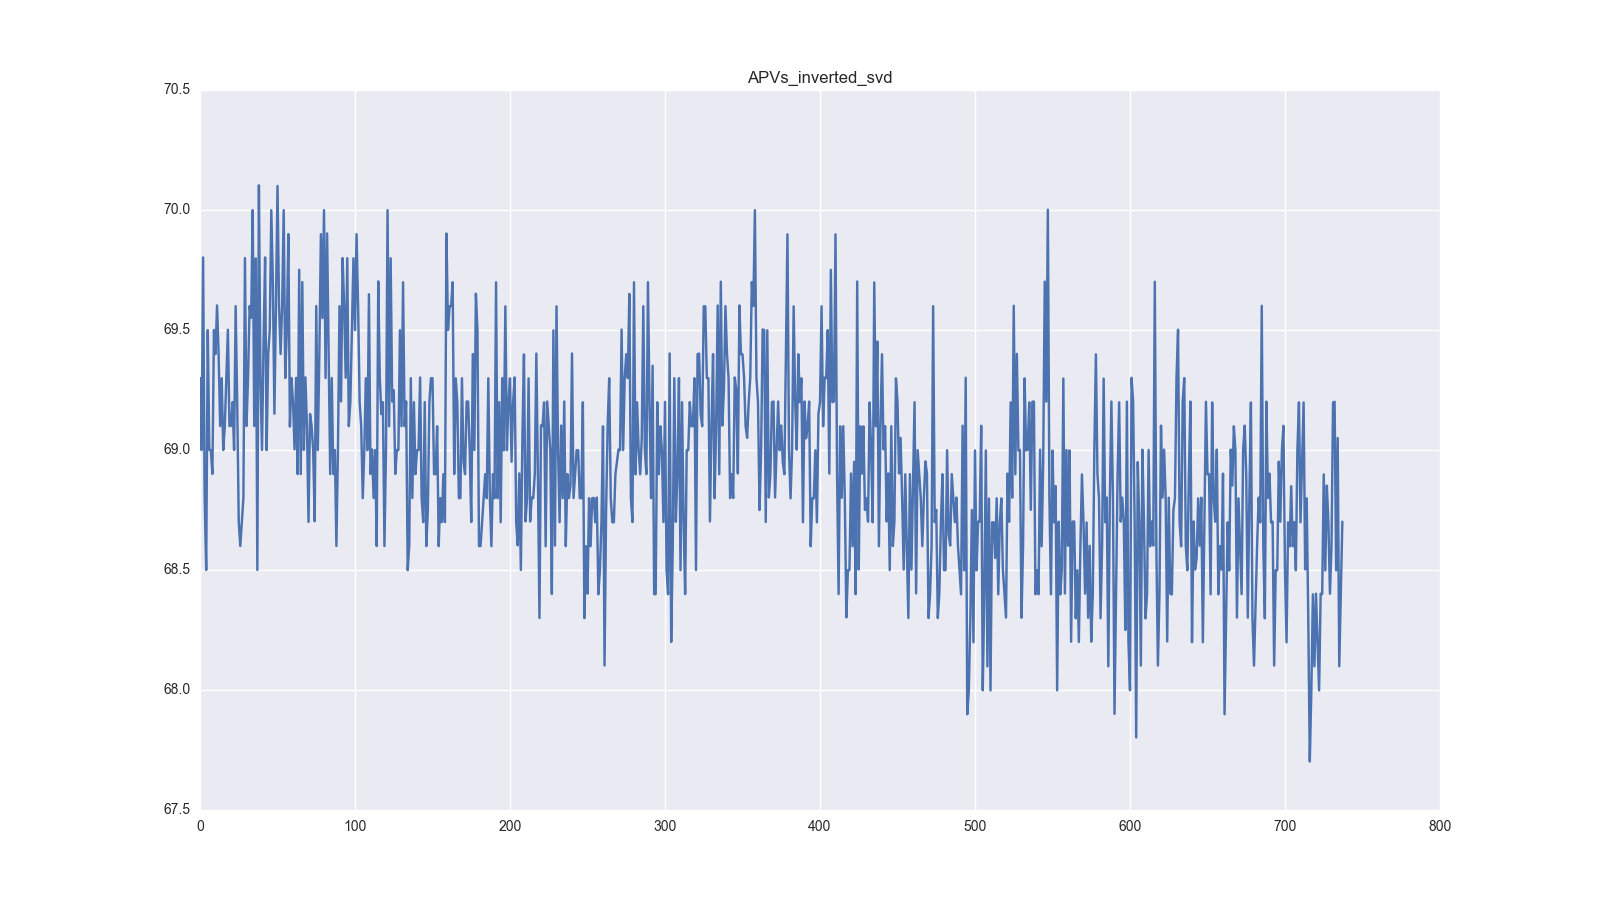
\includegraphics[width=\textwidth]{APVs_inverted_svd.png}
            \caption{Inversión de SVD.}
            \label{fig:APVs_inverted_svd}
        \end{subfigure}
        \caption{Datos invertidos de la variable {\em APVs}.}
        \label{fig:APVs_inverted}
    \end{figure}    
    
    Para algunas de las características la eficiencia de la inversión no es tan evidente. Por ejemplo, la serie de {\em H6x} empieza con una secuencia de valores alrededor de \(39.45\) y luego baja para valores alrededor de \(39.30\), como representado en la Figura~\ref{fig:H6x_original}. 
    
    \begin{figure}[h]
        \centering
        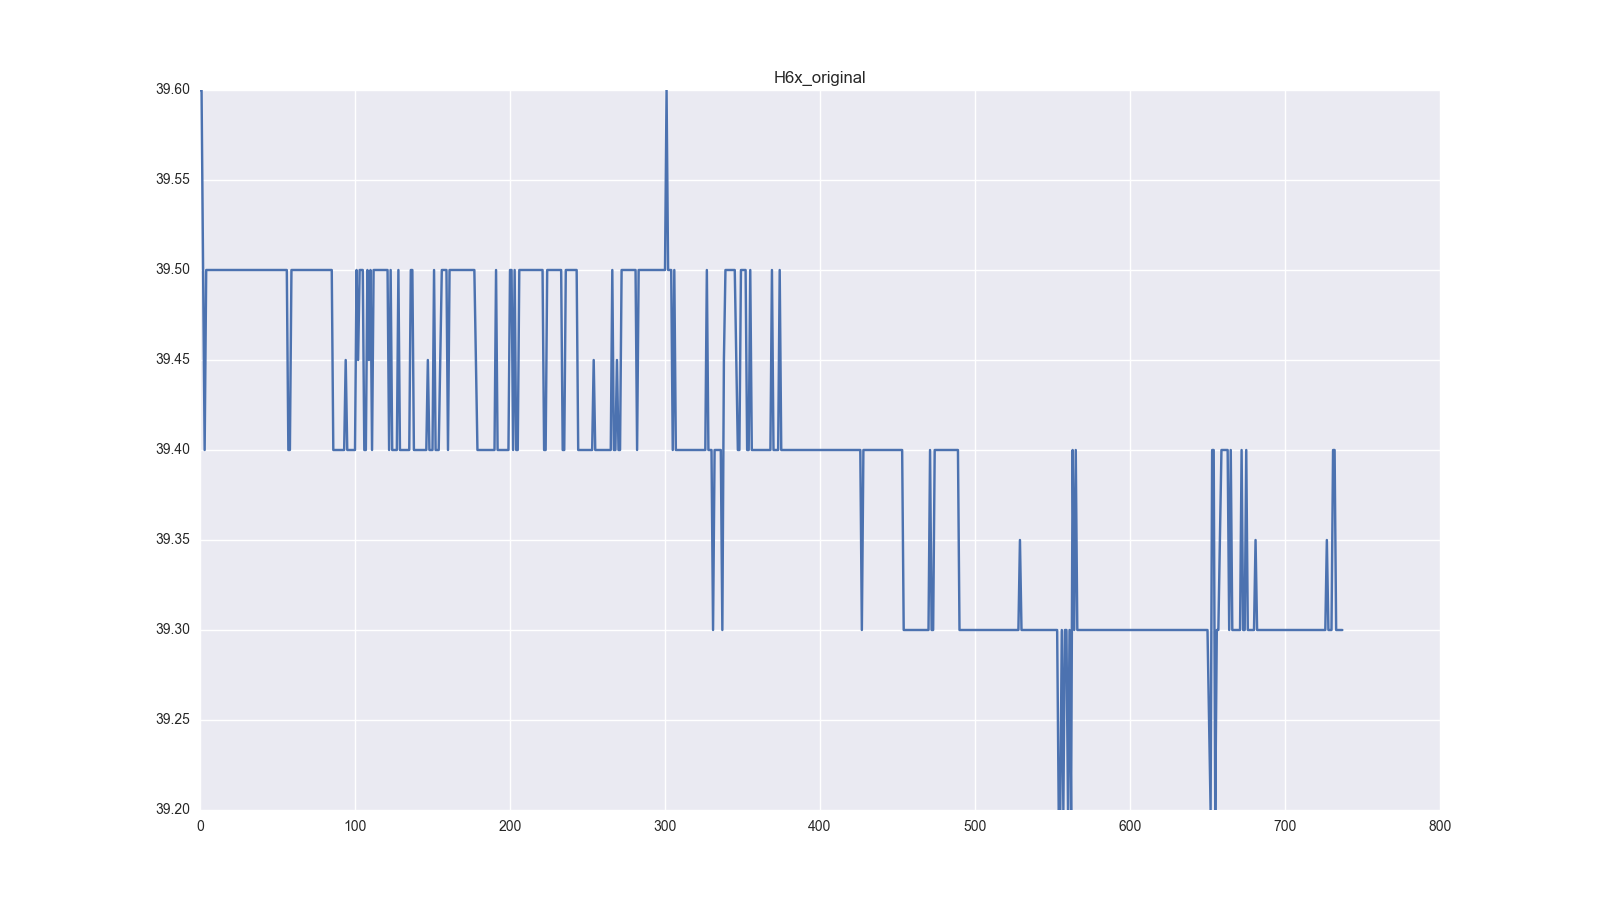
\includegraphics[width=0.7\textwidth]{H6x_original.png}
        \caption{Datos originales de la variable {\em H6x}.}
        \label{fig:H6x_original}
    \end{figure}    
    
    La inversión, sea con NIPALS (Figura~\ref{fig:H6x_inverted_nipals}) o con SVD (Figura~\ref{fig:H6x_inverted_svd}), aunque no tan evidente, también demuestra esa tendencia. Además se puede verificar que los datos invertidos se mantienen dentro del rango de los límites de los valores originales (\(39.20-39.60\)).

    \begin{figure}[h]
        \centering
        \begin{subfigure}[h]{0.49\textwidth}
            \centering
            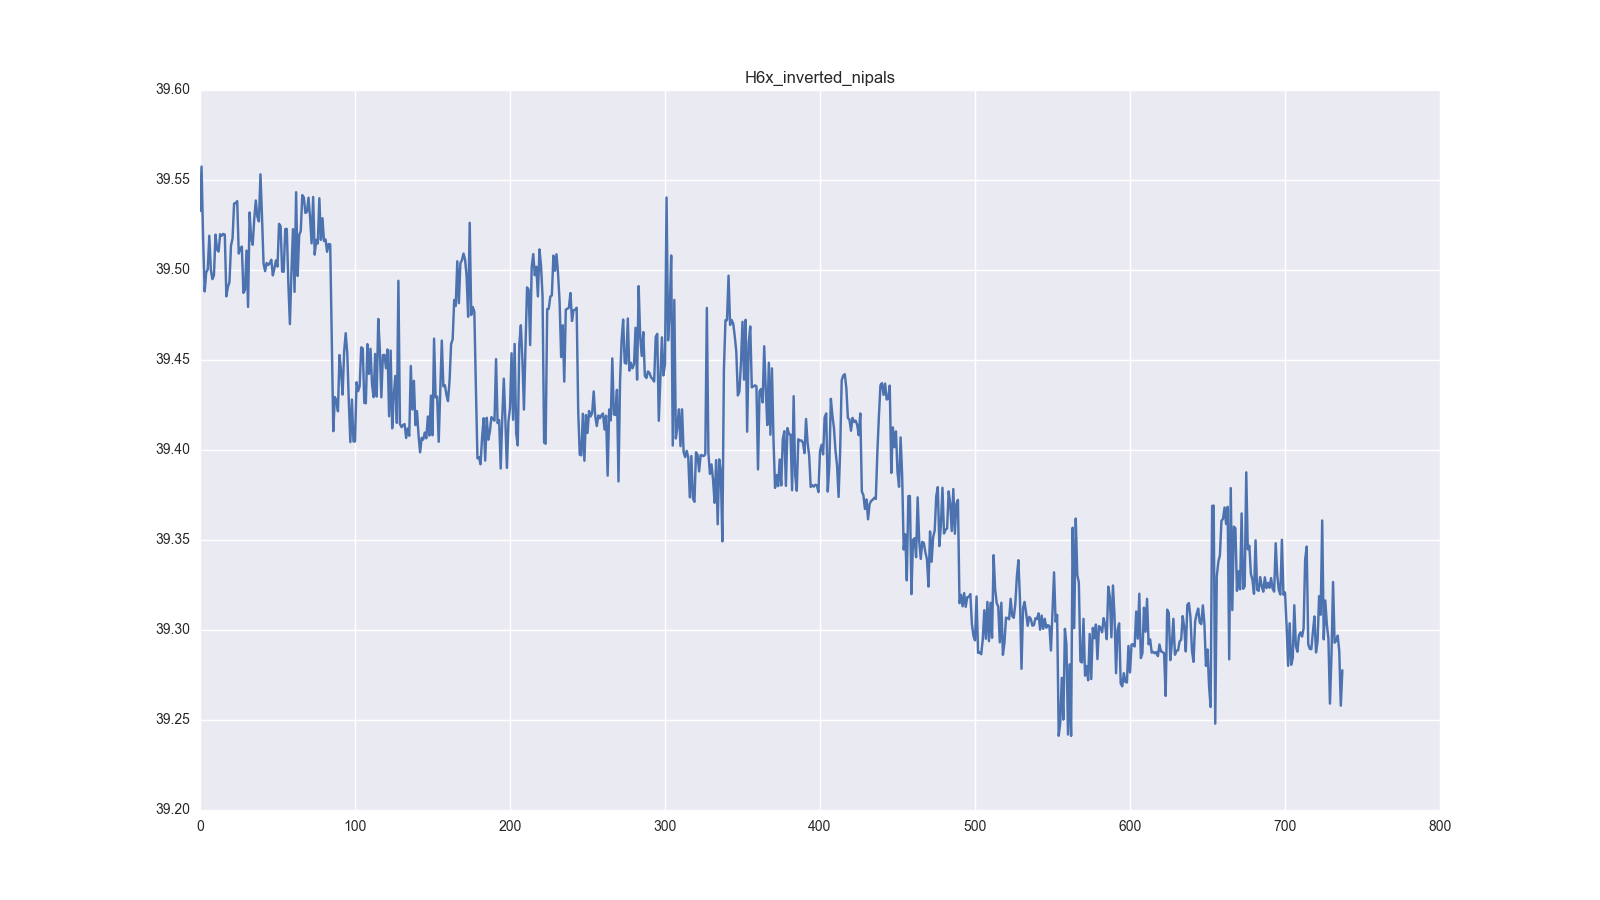
\includegraphics[width=\textwidth]{H6x_inverted_nipals.png}
            \caption{Inversión de NIPALS.}
            \label{fig:H6x_inverted_nipals}
        \end{subfigure}
        \begin{subfigure}[h]{0.49\textwidth}
            \centering
            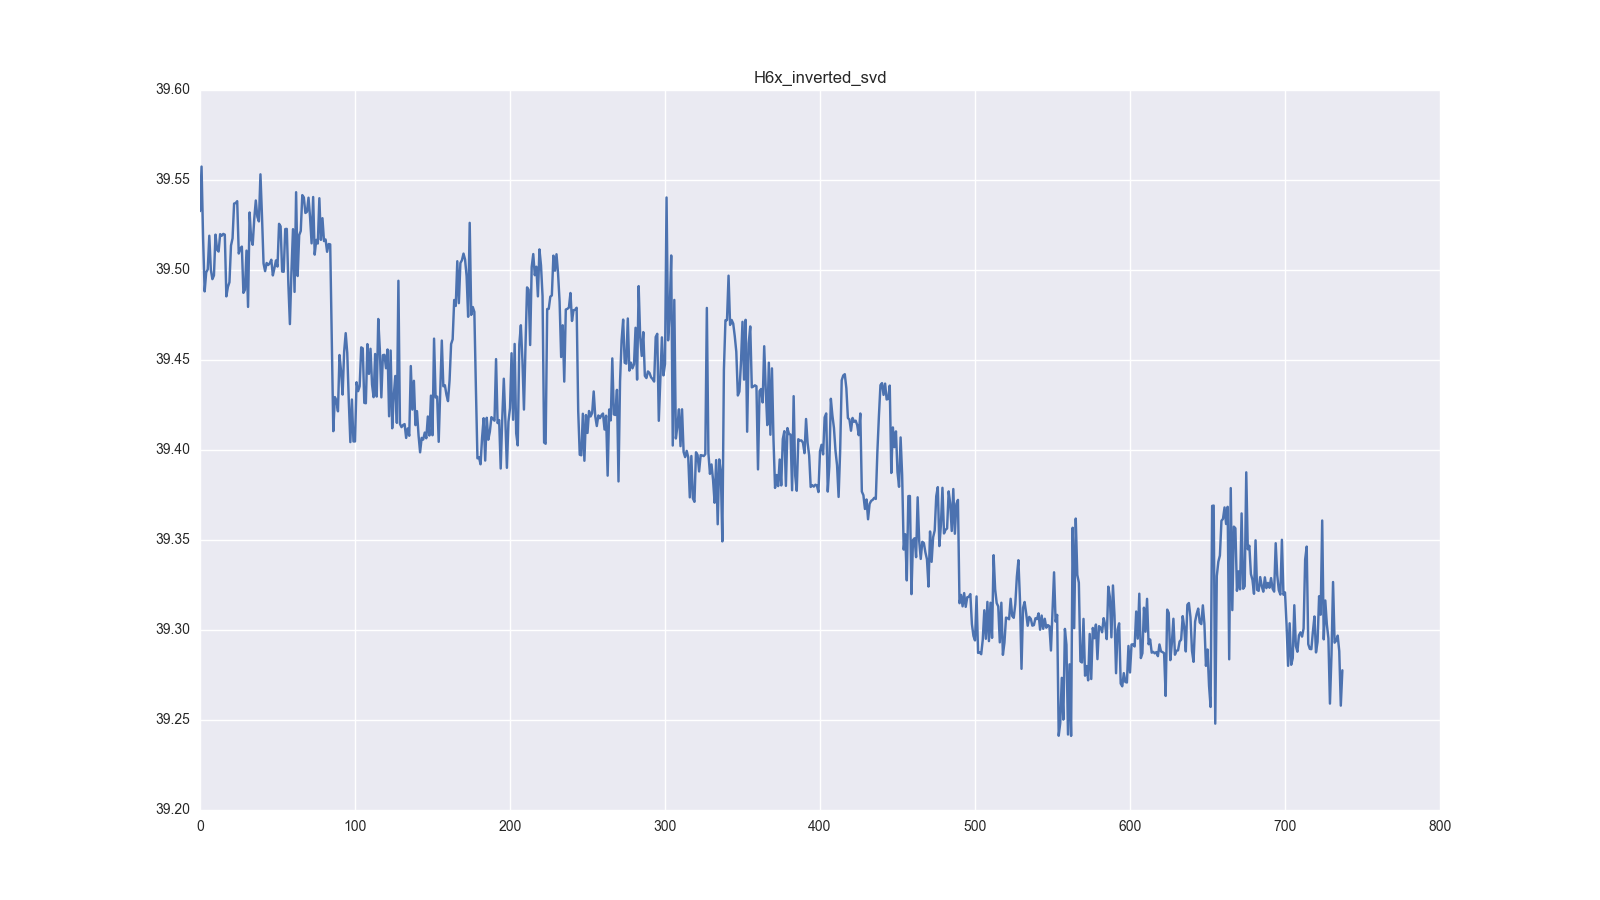
\includegraphics[width=\textwidth]{H6x_inverted_svd.png}
            \caption{Inversión de SVD.}
            \label{fig:H6x_inverted_svd}
        \end{subfigure}
        \caption{Datos invertidos de la variable {\em H6x}.}
        \label{fig:H6x_inverted}
    \end{figure}
    
    Otras características son todavía menos evidentes. Con 5 componentes, los resultados de la inversión de {\em ACPx} son muy poco claros. En un análisis visual, da incluso la sensación de que no corresponde a la misma característica. Véase el gráfico de los datos originales en la Figura~\ref{fig:ACPx_original} y respectiva re-proyección al espacio original en la Figura~\ref{fig:ACPx_inverted}.

    \begin{figure}[h]
        \centering
        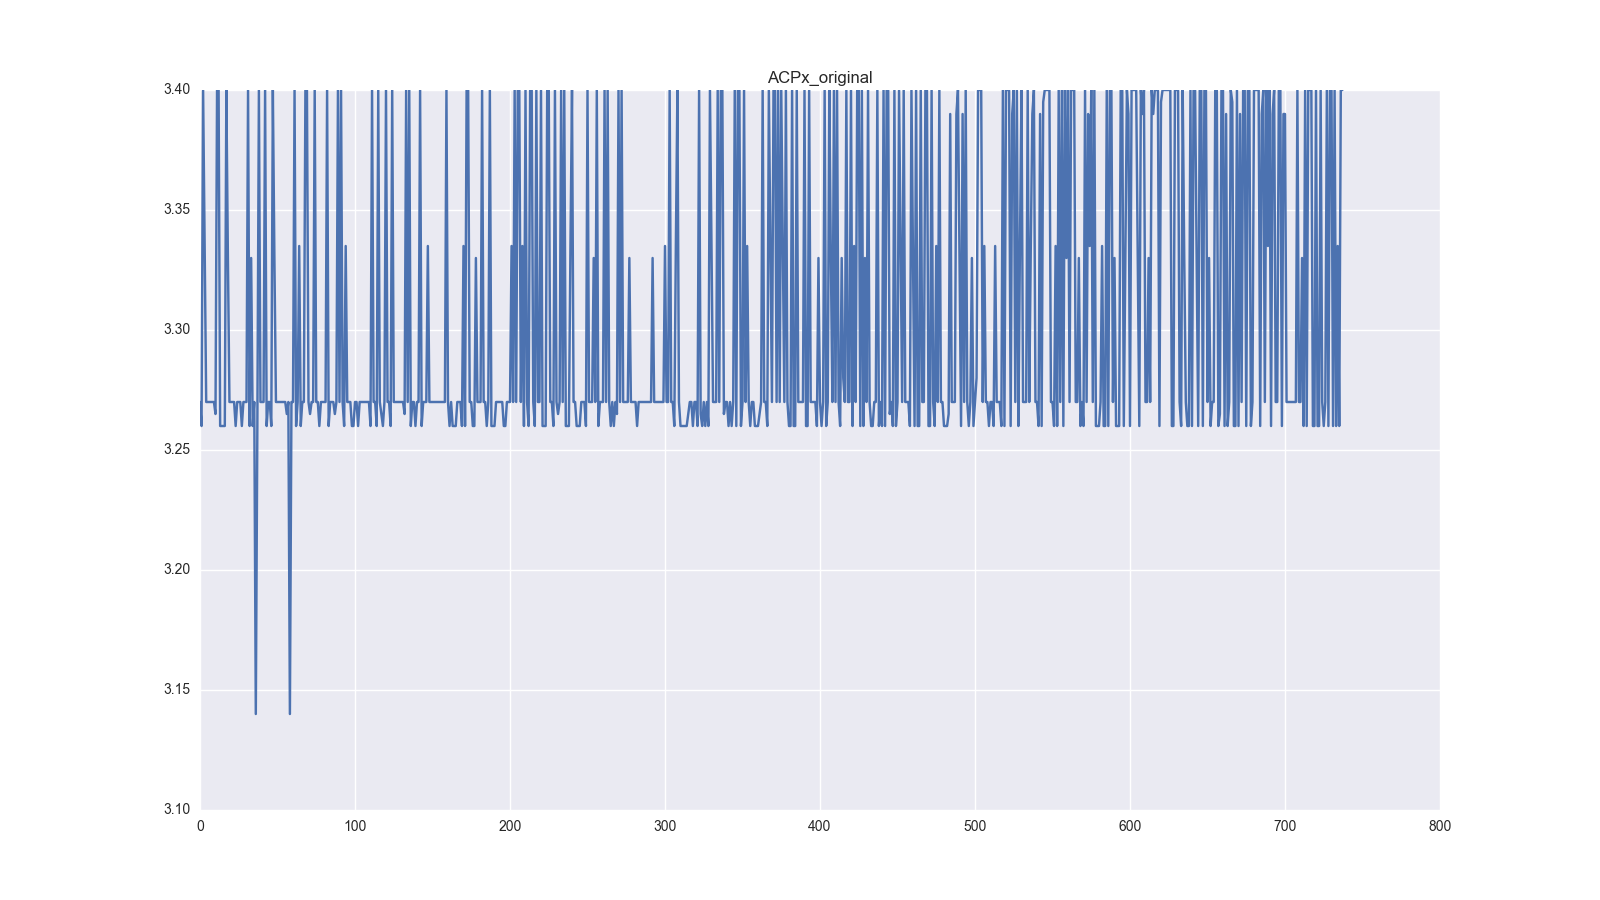
\includegraphics[width=0.7\textwidth]{ACPx_original.png}
        \caption{Datos originales de la variable {\em ACPx}.}
        \label{fig:ACPx_original}
    \end{figure}

    \begin{figure}[h]
        \centering
        \begin{subfigure}[h]{0.49\textwidth}
            \centering
            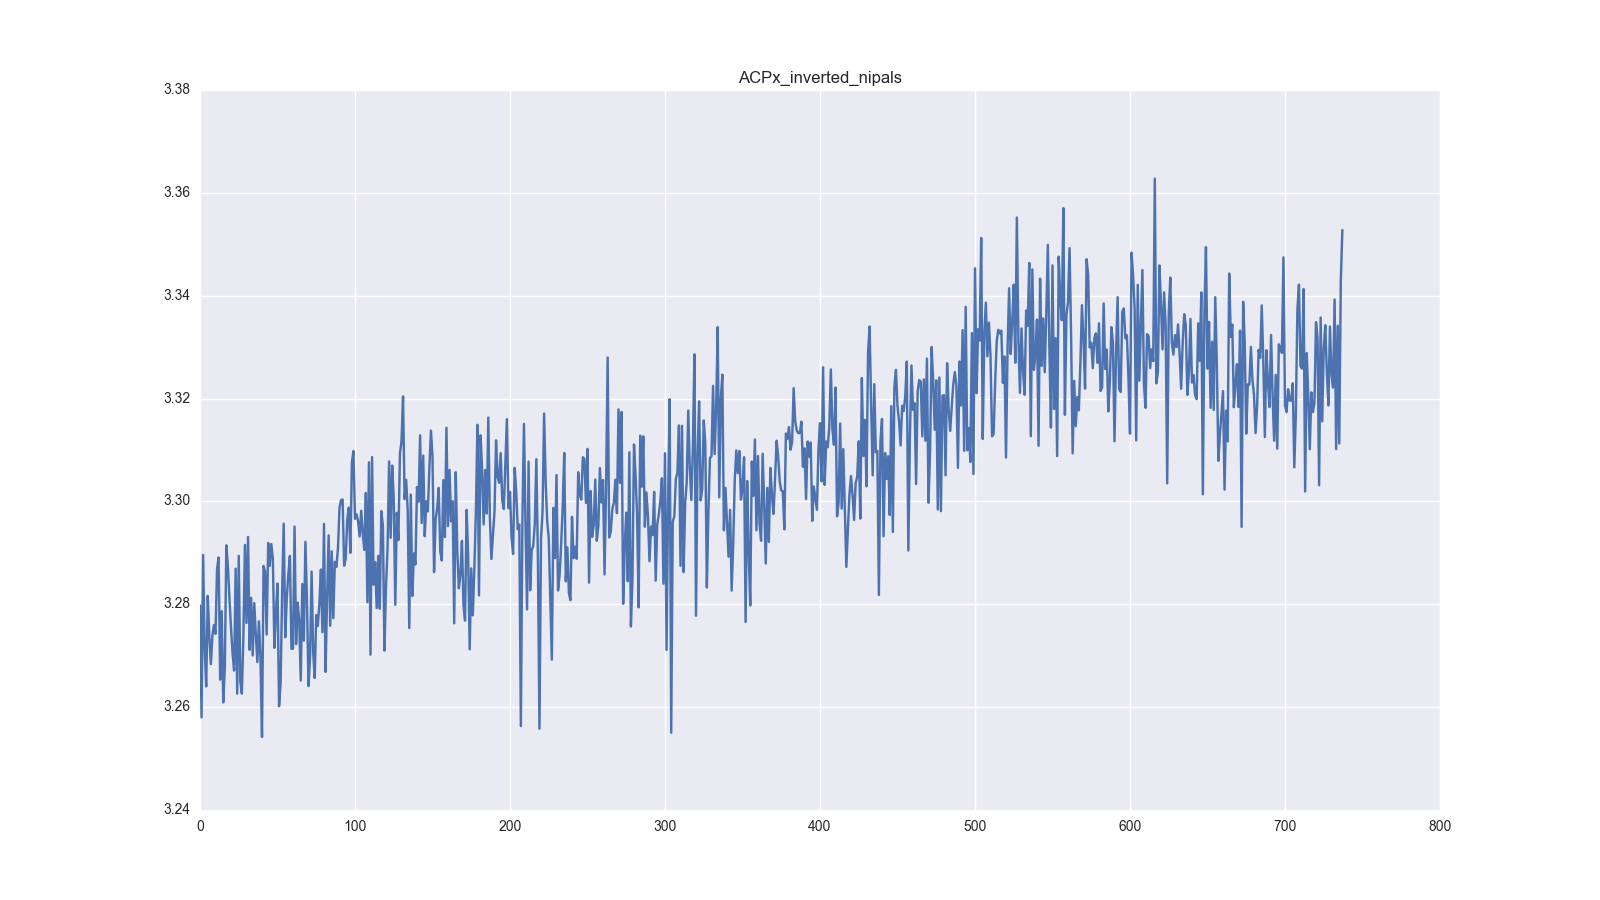
\includegraphics[width=\textwidth]{ACPx_inverted_nipals.png}
            \caption{Inversión de NIPALS.}
            \label{fig:ACPx_inverted_nipals}
        \end{subfigure}
        \begin{subfigure}[h]{0.49\textwidth}
            \centering
            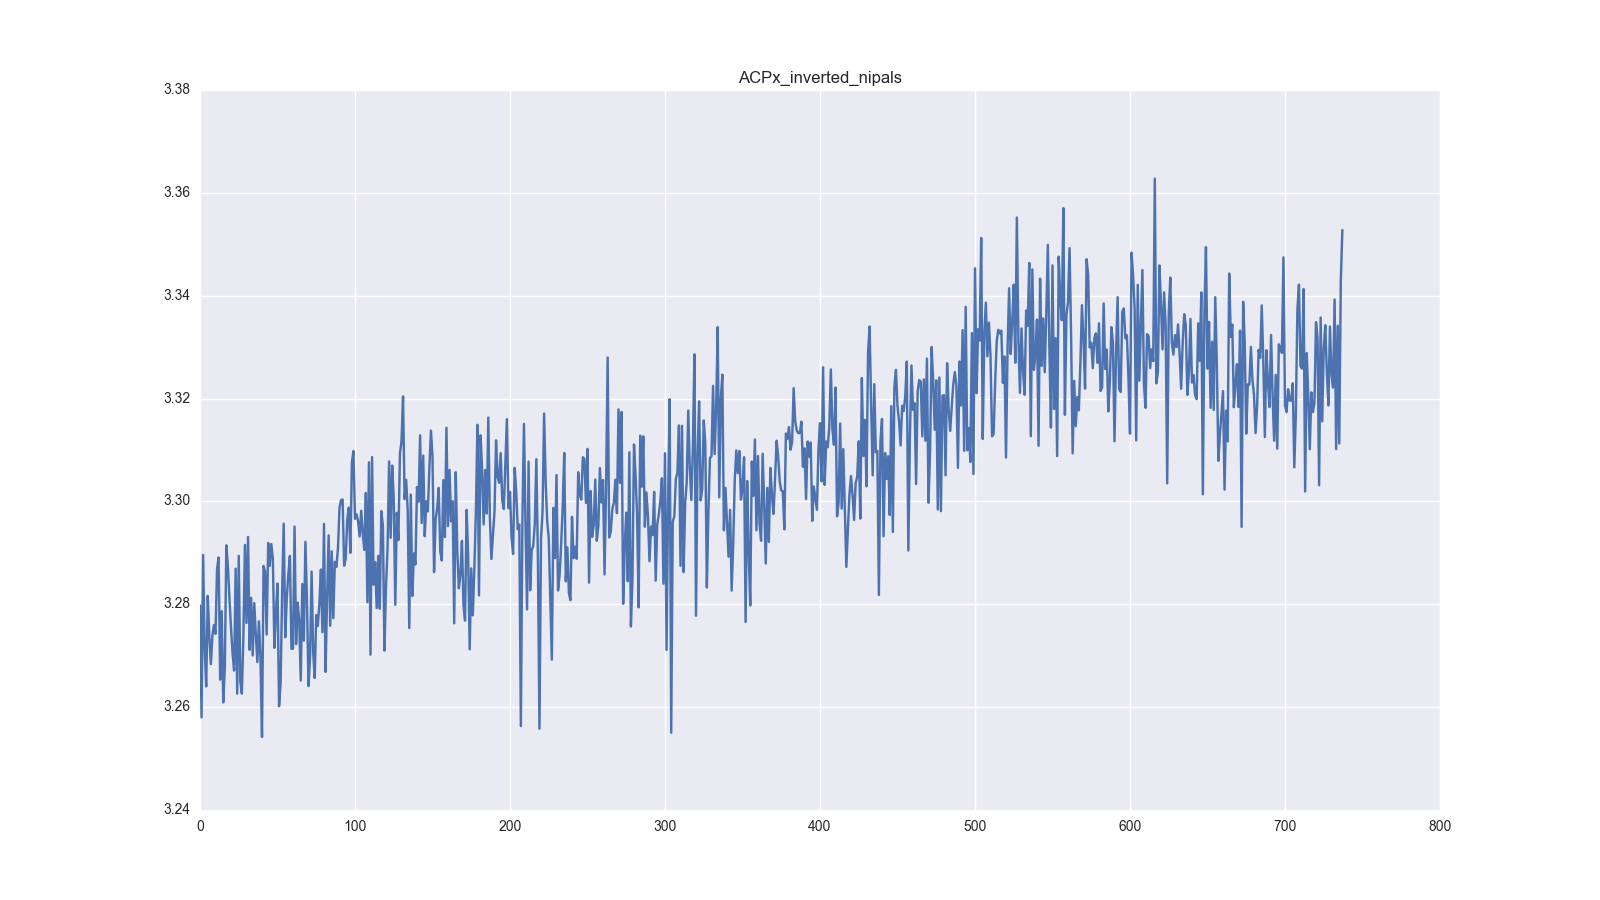
\includegraphics[width=\textwidth]{ACPx_inverted_nipals.png}
            \caption{Inversión de SVD.}
            \label{fig:ACPx_inverted_svd}
        \end{subfigure}
        \caption{Datos invertidos de la variable {\em ACPx}.}
        \label{fig:ACPx_inverted}
    \end{figure}
    
    Aunque parecen datos diferentes, hay algunas propiedades que sí son coherentes, como los límites mínimo y máximo. Los datos originales oscilan principalmente dentro del rango \(3.25-3.40\) y los datos invertidos también. Además, los datos invertidos no contemplan los dos puntos originales que parecen {\em outliers}, con valores de \(\approx 3.14\), probablemente ruido.
    
    En este caso, es importante destacar la elección del numero de componentes. Esa decisión se formalizará más adelante, con el test estadístico. De momento, podemos concluir que, con 5 componentes, los datos invertidos de {\em ACPx} que vemos en la Figura~\ref{fig:ACPx_inverted_nipals} son probablemente la información relevante de la señal. Al final la variabilidad que modelan las últimas componentes es el ruido y quizás en {\em ACPx} hay más ruido que información importante.
    
    Si se calculan más componentes, los resultados se aproximarán más a la realidad, pues se añade a los datos el posible ruido de la señal, que en principio estará contenido en las últimas componentes de la proyección. Sin embargo, aunque el ajuste sea mejor, se pierde generalización del modelo y también la eliminación de ruido. Los resultados de la proyección con 14 componentes se pueden comprobar en la Figura~\ref{fig:ACPx_inverted_nipals_pca14}.
    
    \begin{figure}[H]
        \centering
        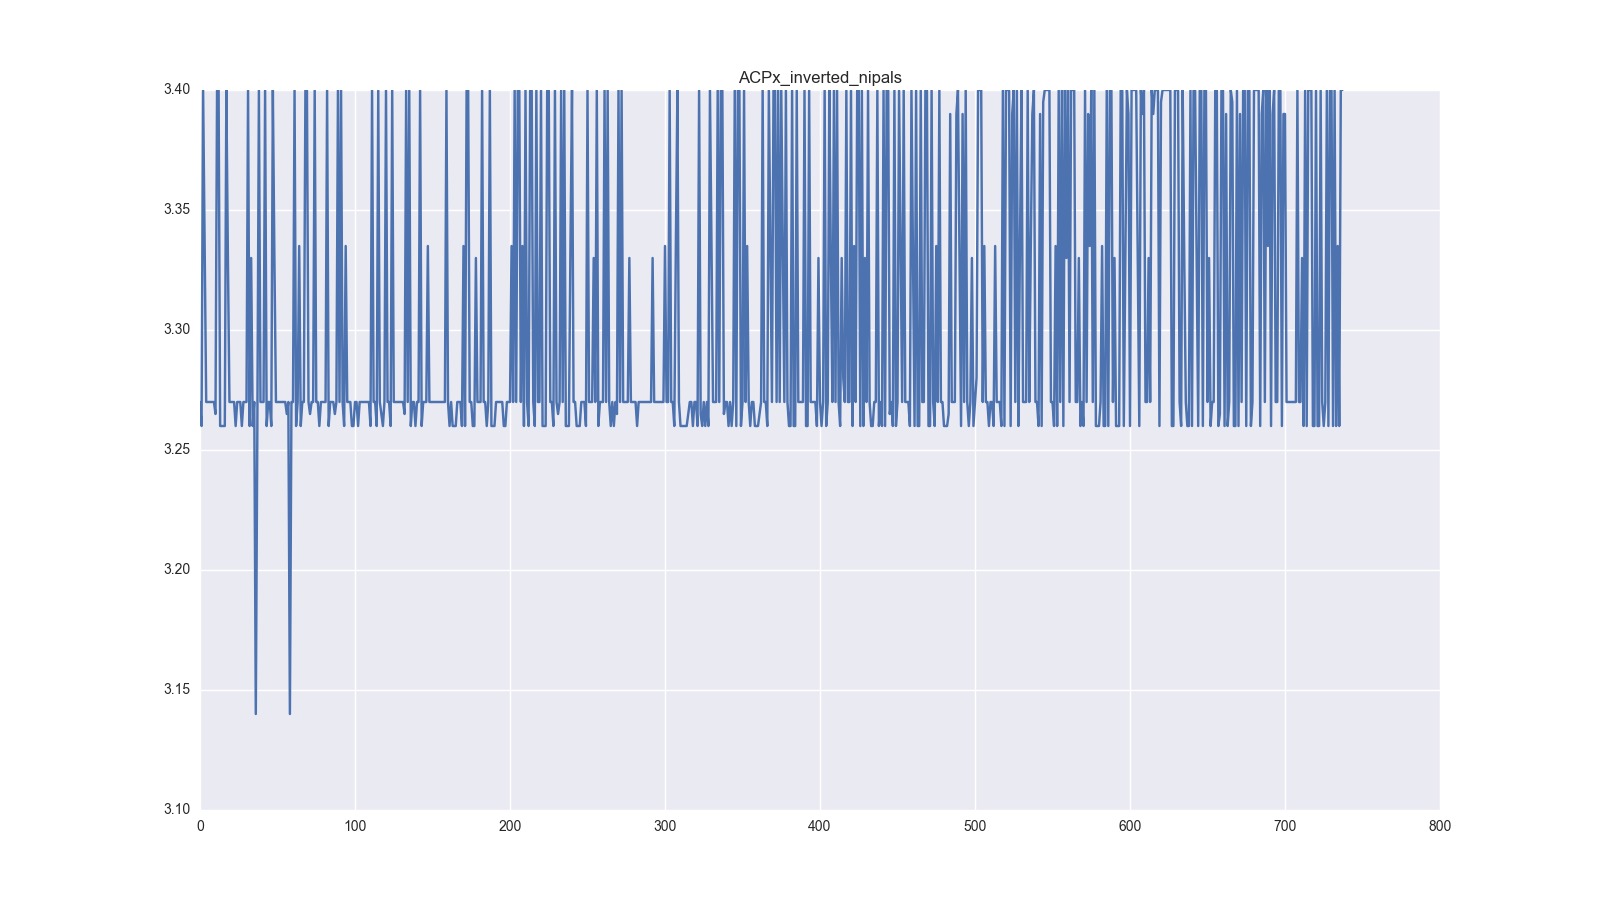
\includegraphics[width=0.7\textwidth]{ACPx_inverted_nipals_pca14.png}
        \caption{Datos invertidos de la variable {\em ACPx} con 14 componentes.}
        \label{fig:ACPx_inverted_nipals_pca14}
    \end{figure}


    % Hotelling T2
    \subsection{Test de hipótesis - Estadístico T-cuadrado de Hotelling}
    Para validar que la inversión de las matrices se está haciendo correctamente necesitamos una medida objetiva que permita comparar estadísticamente las poblaciones original y invertida. Para ello usaremos el estadístico multidimensional \(T^2\) (T-cuadrado) de Hotelling. 
    
    El test \(T^2\) de Hotelling es una generalización del test \(t\) de Student. Para dos muestras (poblaciones), el test \(t\) evalúa las diferencias en las medias de esas poblaciones. El test \(T^2\) se usa cuando las variables son dos o más.

    Las suposiciones del test \(T^2\) de Hotelling para dos poblaciones son:
    \begin{itemize}
    \item cada población sigue una distribución multivariante normal.
    \item las dos poblaciones son independientes.
    \item las dos matrices de varianzas-covarianzas son iguales.
    \end{itemize}
    
    La hipótesis nula es que las medias para todas las variables son iguales. 
    
    Respecto a la implementación, se han usado los algoritmos de test Hotelling \(T^2\) R, con la librería {\tt Hotelling}. El Código~\ref{lst:t2_test} es un ejemplo de uso de la librería.

    \begin{lstlisting}[language=S, caption=Test \(T^2\) de Hotelling en R., label={lst:t2_test}]
> res = hotelling.test(x = data, y = inverted_data)
> print(res)
Test stat:  0.072321 
Numerator df:  14 
Denominator df:  119782 
P-value:  1
    \end{lstlisting}
    
    Si el valor del estadístico es significativo (valor alto) significa que ha encontrado bastantes diferencias entre las poblaciones, por lo que podemos rechazar la hipótesis nula. En el caso demostrado en el Código~\ref{lst:t2_test}, el resultado del estadístico es poco significativo (cercano a cero), así que podemos aceptar la hipótesis nula. La interpretación es que las poblaciones {\tt data} y {\tt inverted\_data} son iguales, con un grado de confianza alta ({\tt p-value=1}). 
    
    Se ha aplicado el test \(T^2\) de Hotelling exhaustivamente para los varios números de componentes posibles. Los resultados se encuentran en la tabla~\ref{table:t2_test}.
    
    \begin{table}
         \centering
         \begin{tabular}{|c|c|c|} 
             \hline
             Componentes & Hotelling \(T^2\) & p-valor \\ [0.5ex] 
             \hline\hline
             1 & 0.020809 & 1 \\ 
             \hline
             2 & 0.063641 & 1 \\ 
             \hline
             3 & 0.01215 & 1 \\ 
             \hline
             4 & 0.013919 & 1 \\ 
             \hline
             5 & 0.020096 & 1 \\ 
             \hline
             6 & 0.077881 & 1 \\ 
             \hline
             7 & 0.031675 & 1 \\ 
             \hline
             8 & 0.00012993 & 1 \\ 
             \hline
             9 & 0.20037 & 0.9994 \\ 
             \hline
             10 & 0.029146 & 1 \\ 
             \hline
             11 & 0.16149 & 0.9998 \\ 
             \hline
             12 & 0.08343 & 1 \\ 
             \hline
             13 & 0.0024538 & 1 \\ 
             \hline
             14 & 0.13956 & 0.9999 \\ 
             \hline
        \end{tabular}
        \caption{Test \(T^2\) de Hotelling para los varios números de componentes.}
        \label{table:t2_test}
    \end{table}
    
    Se ha usado un pequeño factor aleatorio con distribución normal para ocupar valores vacíos en determinadas variables. Por esa razón los resultados pueden variar y ser algo incoherentes (por ejemplo, con 9 componentes tenemos mayor valor del estadístico que con 1 componente). De todas formas, el objetivo de este análisis exhaustivo es verificar que la inversión de NIPALS es correcta - podemos afirmar que sí, pues el estadístico presenta valores poco significativos y los p-valor son altos.
    
    Aunque los p-valor sean altos (cercanos a 1), se detecta una tendencia para ser inferior a 1 a partir de un determinado numero de componentes (en la tabla ~\ref{table:t2_test} sería a partir de 9 componentes que el p-valor empieza a dar señales de bajada). Probablemente, esa variación se debe a la introducción del ruido a partir de ese numero de componentes. En base a este estudio, se ha decidido usar 5 componentes para el cálculo de PCA.

    % Gaussiana
    \subsection{Simulación con distribución Gaussiana}
    El primer acercamiento de simulación de datos se hizo usando la distribución normal o Gaussiana. El algoritmo es: para cada componente, se calcula la media y variación típica y, a partir de estos, se genera una nueva serie con distribución gaussiana (ver código~\ref{lst:gaussian_simulation}).
    
    \begin{lstlisting}[language=Python, caption=Simulación con distribución Gaussiana., label={lst:gaussian_simulation}]
mus = np.mean(nipals_T, axis=0)
sigmas = np.std(nipals_T, axis=0)

generated_gaussian = np.zeros((GAUSSIAN_SIZE, N_COMPONENTS))
for i in range(N_COMPONENTS):
    # calculate normal distribution by component and store it in column i
    generated_gaussian[:, i] = np.random.normal(mus[i], sigmas[i], GAUSSIAN_SIZE)
    \end{lstlisting}
    
    La Figura~\ref{fig:component_0_gaussian} da una idea gráfica de la simulación con distribución Gaussiana para la componente 1. En verde vemos los datos de la componente y en azul los datos generados. Las líneas gris representan la media, mínimo, máximo y algunas desviaciones típicas. Los datos generados se mantienen dentro de los límites de la serie de la componente.

    \begin{figure}[H]
        \centering
        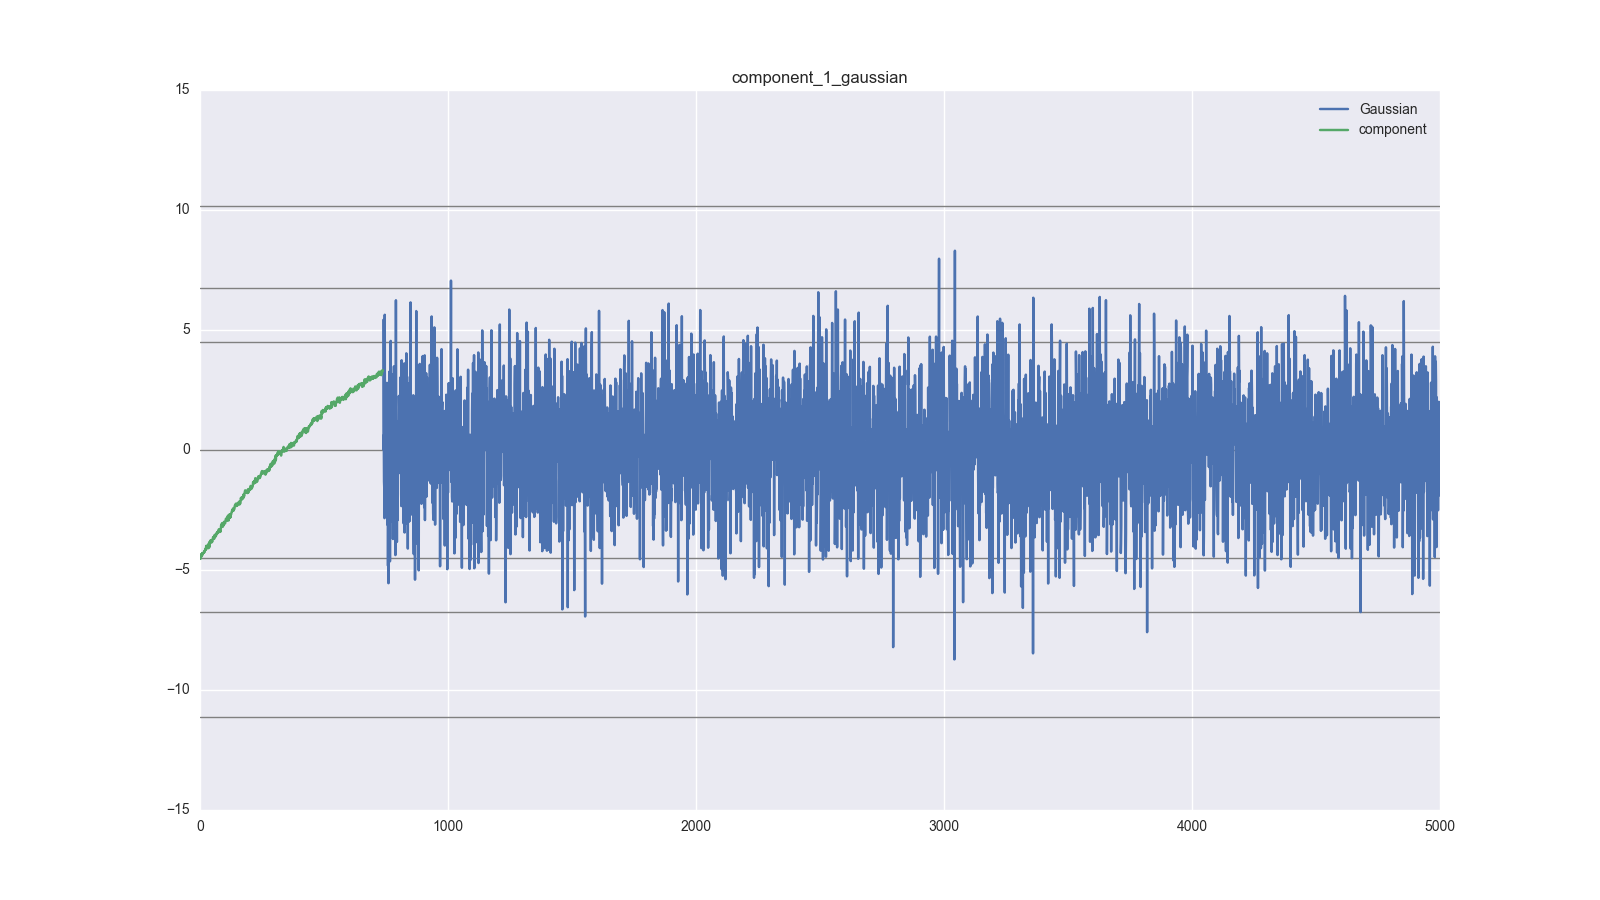
\includegraphics[width=0.7\textwidth]{component_1_gaussian.png}
        \caption{Datos originales y simulados de la componente 1.}
        \label{fig:component_0_gaussian}
    \end{figure}   
    
    Las simulaciones para las demás componentes se representan en la secuencia de gráficos de la Figura~\ref{fig:component_gaussian}.
    
    \begin{figure}[H]
        \centering
        \begin{subfigure}[h]{0.49\textwidth}
            \centering
            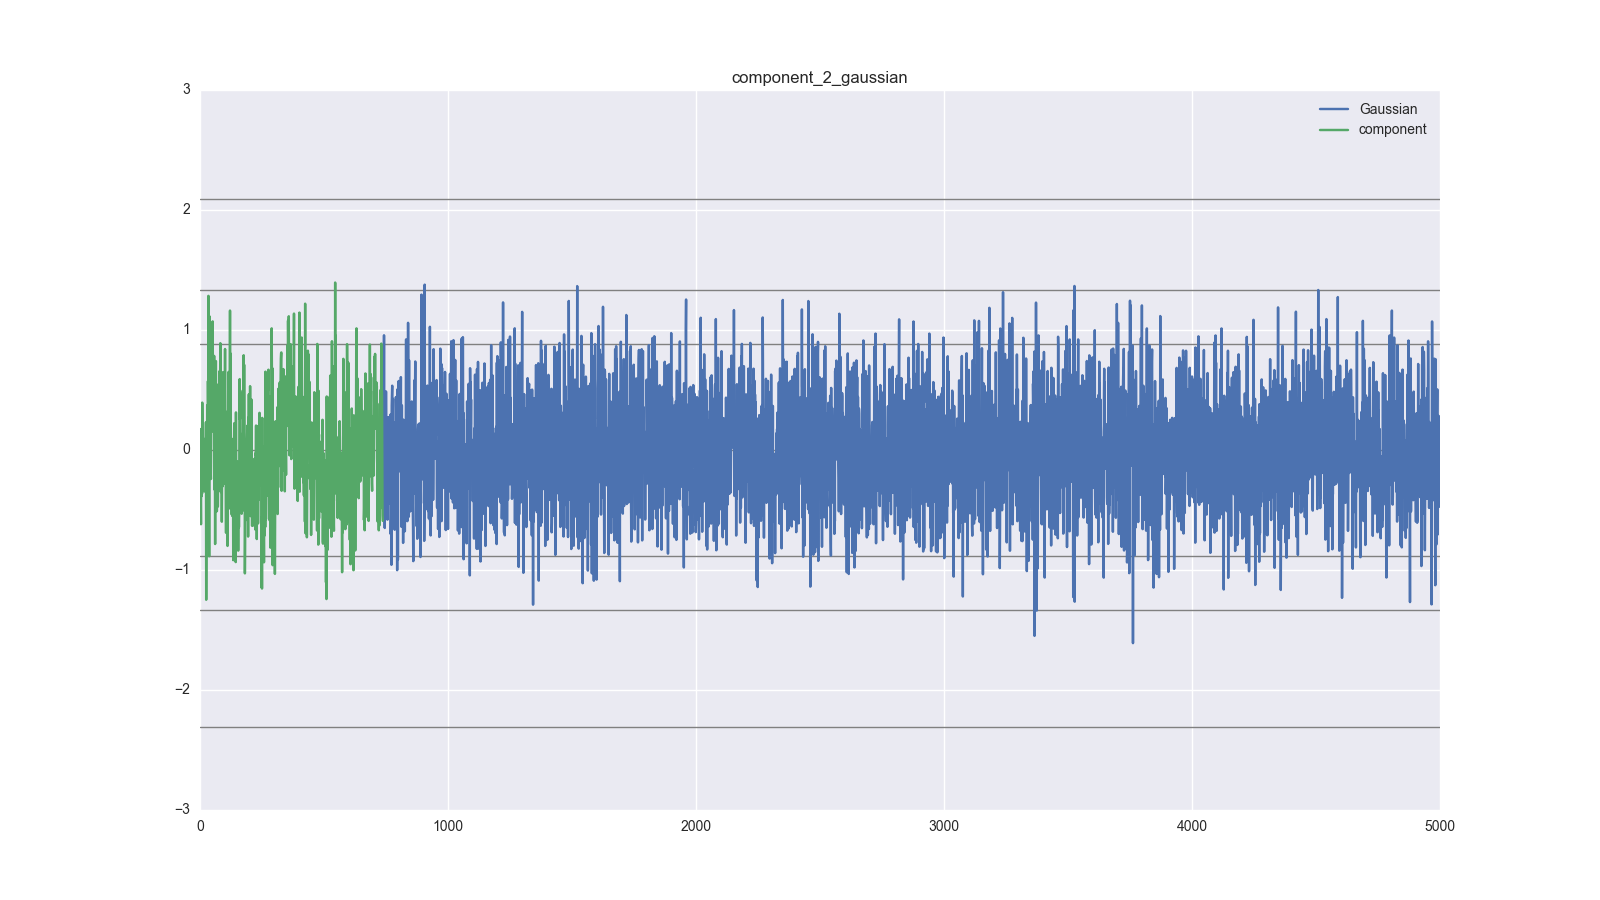
\includegraphics[width=\textwidth]{component_2_gaussian.png}
            \caption{Componente 2.}
            \label{fig:component_2_gaussian}
        \end{subfigure}
        \begin{subfigure}[h]{0.49\textwidth}
            \centering
            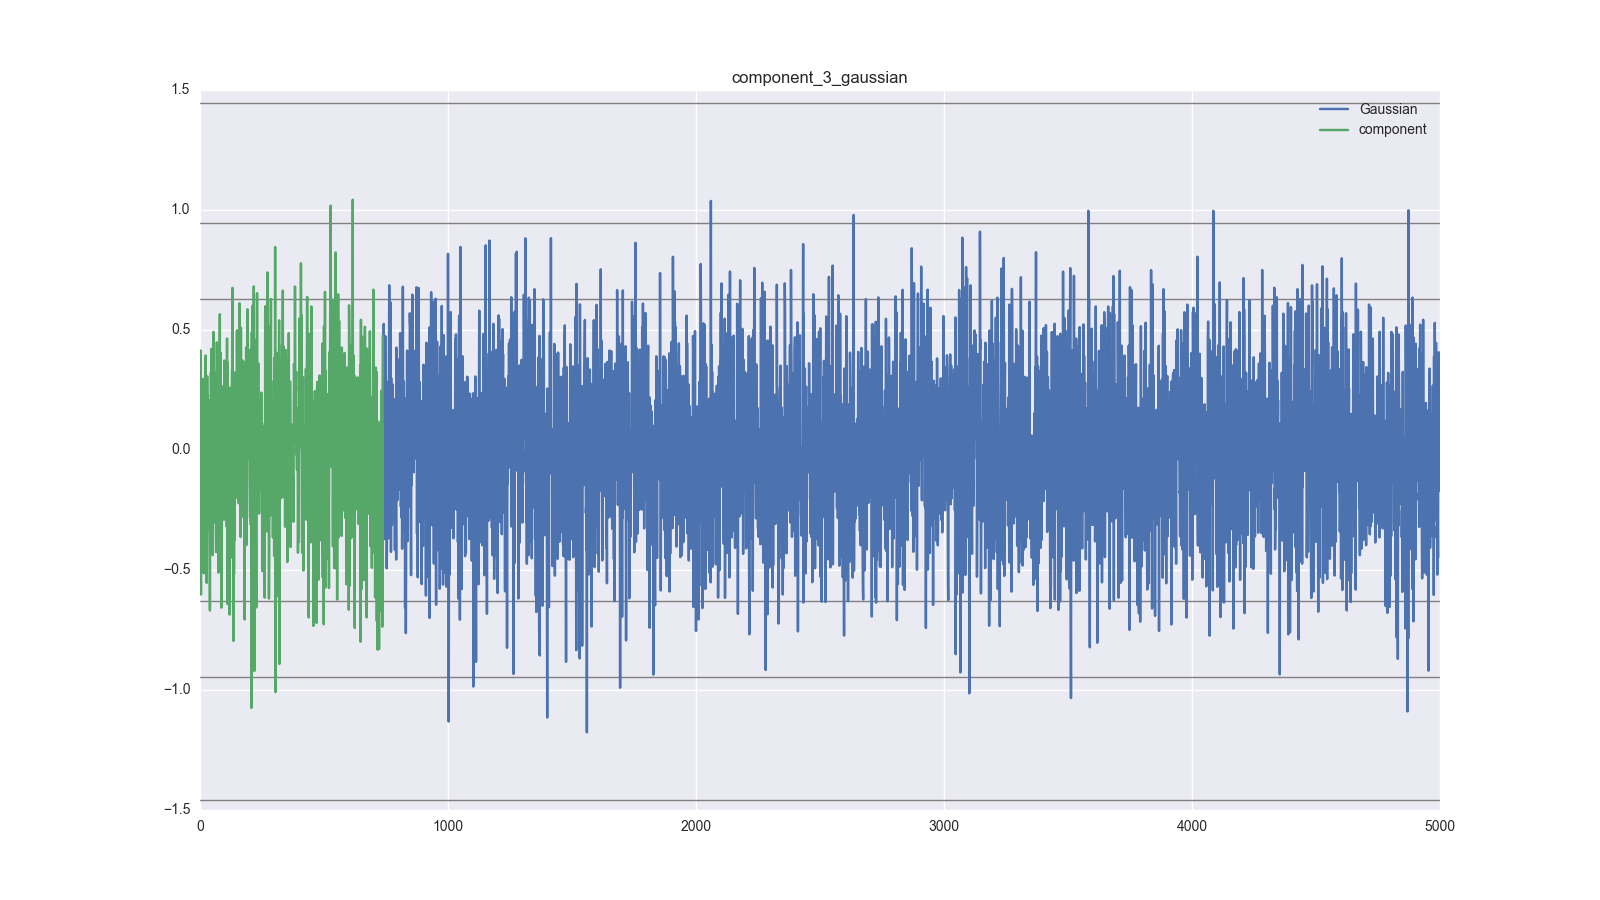
\includegraphics[width=\textwidth]{component_3_gaussian.png}
            \caption{Componente 3.}
            \label{fig:component_3_gaussian}
        \end{subfigure}
        \begin{subfigure}[h]{0.49\textwidth}
            \centering
            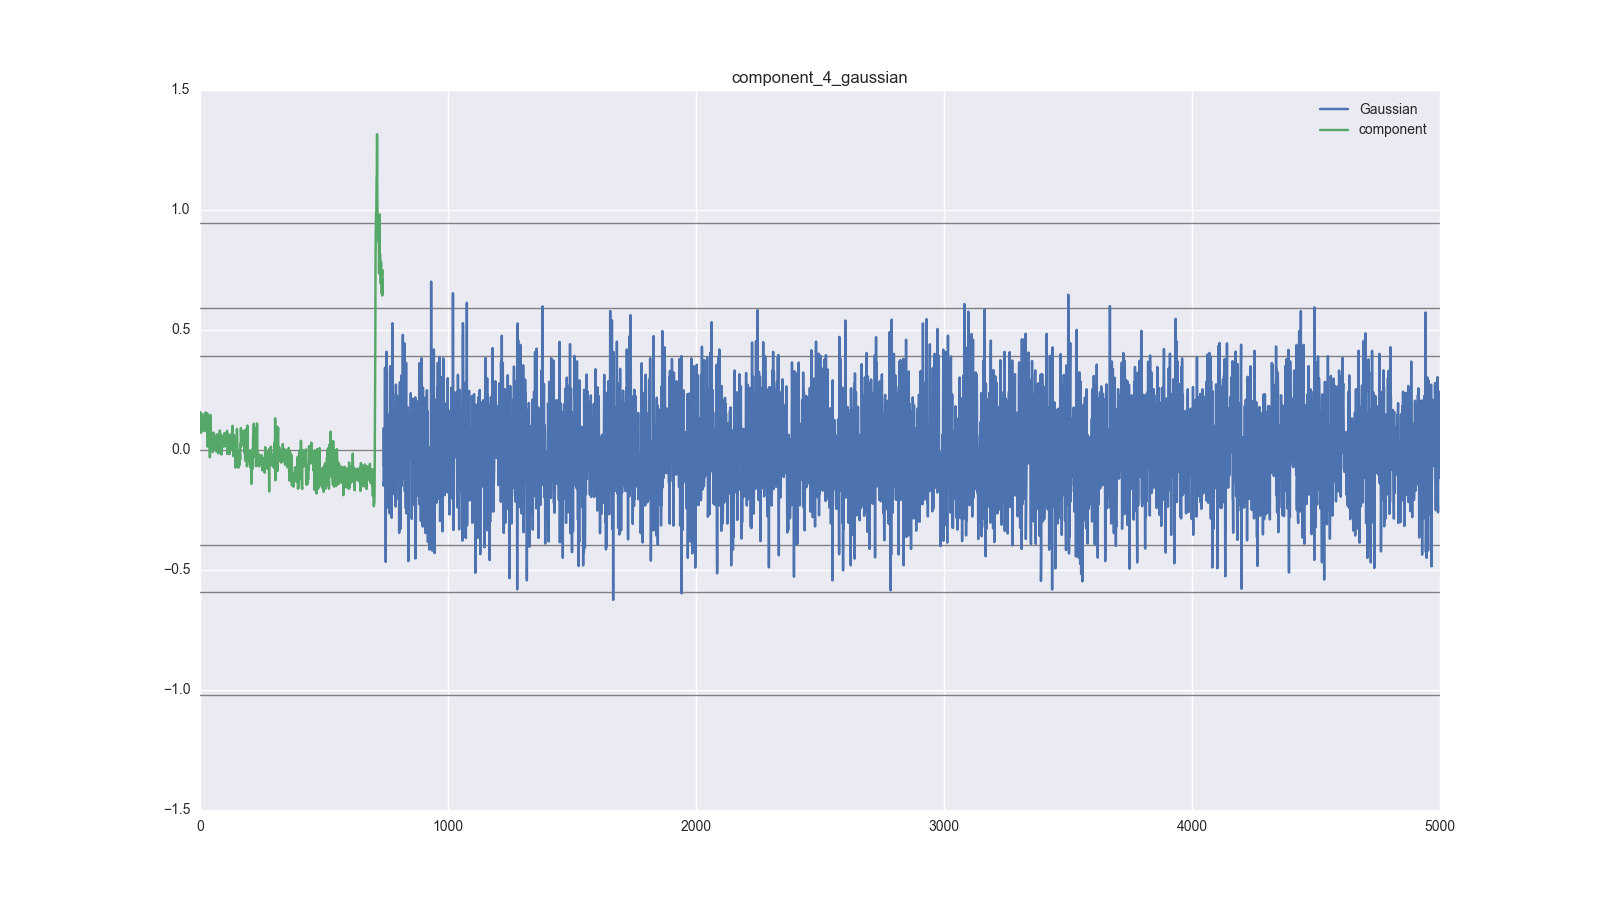
\includegraphics[width=\textwidth]{component_4_gaussian.png}
            \caption{Componente 4.}
            \label{fig:component_4_gaussian}
        \end{subfigure}
        \begin{subfigure}[h]{0.49\textwidth}
            \centering
            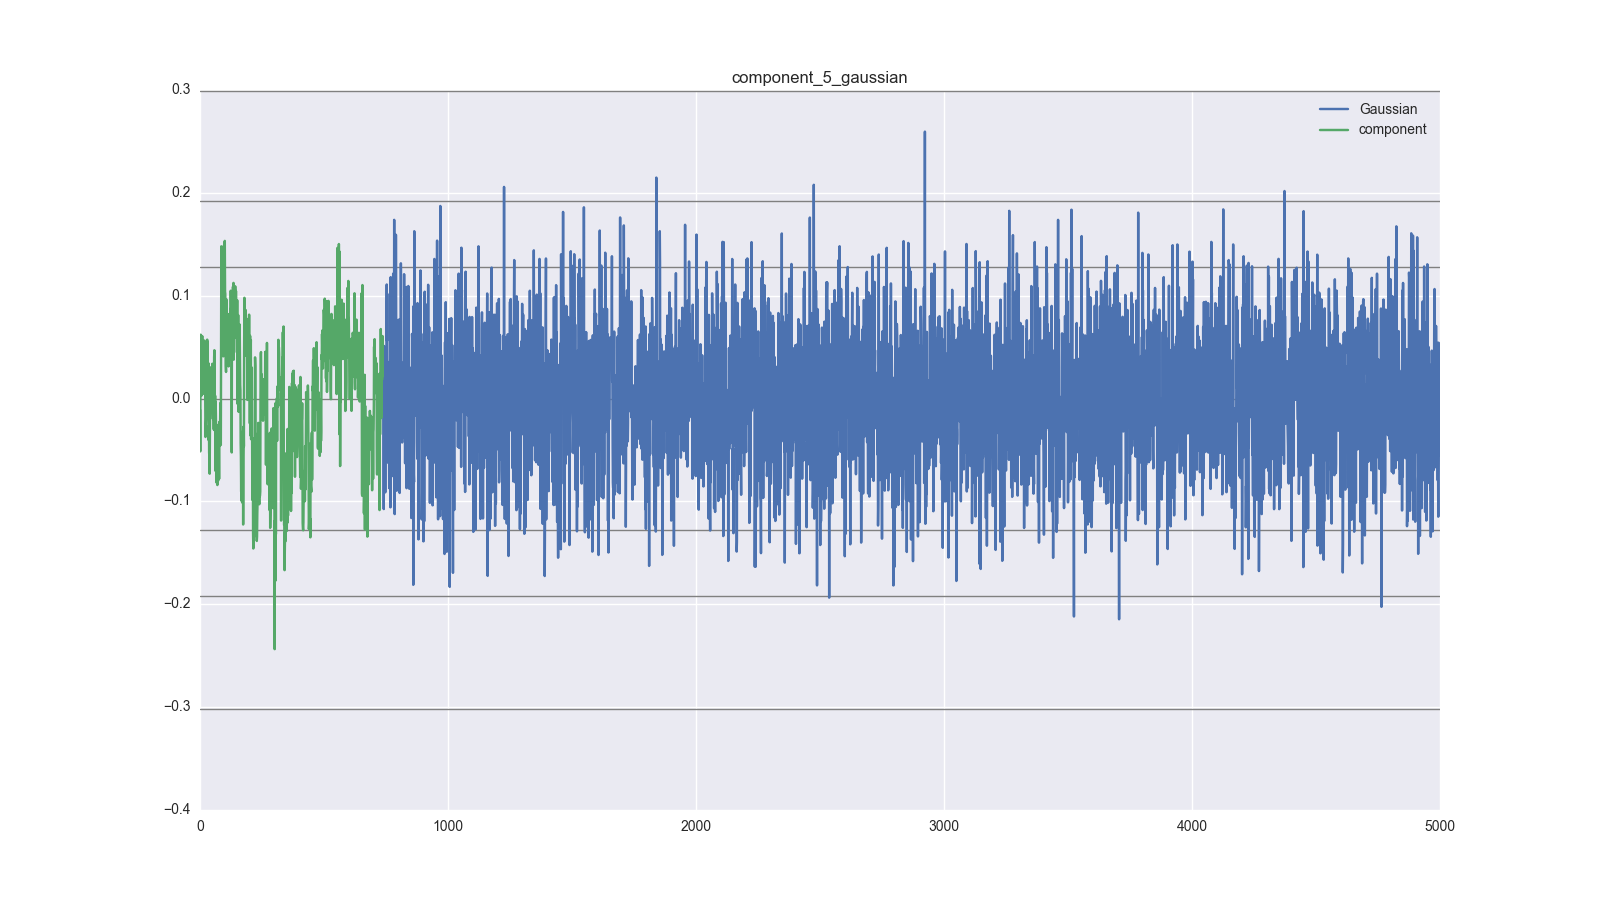
\includegraphics[width=\textwidth]{component_5_gaussian.png}
            \caption{Componente 5.}
            \label{fig:component_5_gaussian}
        \end{subfigure}
        \caption{Datos originales y simulados de las componentes.}
        \label{fig:component_gaussian}
    \end{figure}
 
    Una vez generados los nuevos datos de las componentes, se re-proyectan al espacio original y se obtiene la nueva población multivariante, simulada. La Figura~\ref{fig:inverse_gaussian_APHu} da un ejemplo de la re-proyección usando la simulación Gaussiana, para la variable {\em APHu}.
    
    \begin{figure}[H]
        \centering
        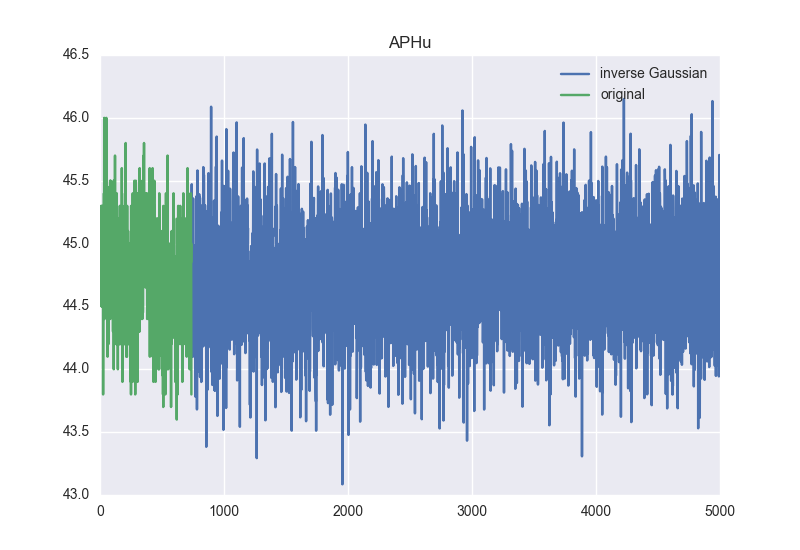
\includegraphics[width=0.7\textwidth]{inverse_gaussian_APHu.png}
        \caption{Datos originales y simulados de la variable {\em APHu}.}
        \label{fig:inverse_gaussian_APHu}
    \end{figure}       
    
    Sometiendo los nuevos datos al test \(T^2\) de Hotelling, se verifica que es igual a la población original (código~\ref{lst:gaussian_simulation}). El estadístico tiene un valor poco significativo de \(0.037391\) y el p-valor es \(1\), así que la hipótesis nula (las poblaciones son diferentes) puede ser rechazada.
    
    \begin{lstlisting}[language=S, caption=Test \(T^2\) de Hotelling para la simulación con distribución Gaussiana., label={lst:gaussian_simulation}]
> res <- hotelling.test(x = data, y = inverted_data_gaussian)
> print(res)
Test stat:  0.037391 
Numerator df:  14 
Denominator df:  100723 
P-value:  1 
    \end{lstlisting}
    
    Para validar el correcto funcionamiento del test implementado en {\tt hotelling.test}, se ha generado una serie con valores aleatorios con distribución no normal. Con esto, es de esperar que el estadístico adopte valores significativos y que el p-valor se aleje de \(1\). El código~\ref{lst:non_normal_simulation} corrobora esa expectativa.
   
    \begin{lstlisting}[language=S, caption=Test \(T^2\) de Hotelling para la simulación con distribución no normal., label={lst:non_normal_simulation}]
> res <- hotelling.test(x = data, y = inverted_data_non_normal)
> print(res)
Test stat:  719.81 
Numerator df:  14 
Denominator df:  100723 
P-value:  0 
    \end{lstlisting}

    La simulación con distribución Gaussiana constituye la base de nuestro estudio para la simulación de datos. Asumimos, a partir de ahora, que las componentes simuladas con distribución Gaussiana, al ser re-proyectados al espacio original, producen una nueva población que es similar a la original. Esta base sustenta algunas decisiones de los próximos capítulos y, por consiguiente, los resultados finales del estudio.
        
    % ARIMA
    \section{ARIMA}
    Una vez determinado el numero de componentes a usar y realizadas las primeras simulaciones con distribución normal, el siguiente paso consiste en construir series temporales sobre cada una de las componentes para simular con cierto sentido temporal. El objetivo es que los datos generados tengan forma de serie temporal. Para poder aplicar los modelos ARIMA introducidos anteriormente hay que preparar y estudiar los datos previamente. Una vez preparada la serie, se pasa a la predicción del comportamiento futuro, la simulación propiamente dicha.
        
        % Preparación
        \subsection{Preparación de la serie temporal}
        Las mediciones de los sensores son dadas a periodos temporales que no siempre son regulares. Los datos de los sensores tienen muchos huecos, es decir, períodos largos sin mediciones. Además la frecuencia de mediciones no es constante, a veces es cada 10 segundos y otras cada minuto. La primera consideración para el análisis de series temporales es que éstas deben ser un conjunto de datos observados a periodos fijos. 
        
        La preparación consiste en transformar la serie para que sea homogénea en los periodos de observaciones. Se verifica también que las mediciones son muy discrepantes en días diferentes, potencialmente por corresponder a diferentes pruebas en las máquinas industriales. Para simular un proceso productivo continuo, no tiene sentido juntar los varios días si hay demasiada discrepancia entre ellos; unirlos supondría hacer asociaciones potencialmente muy fuertes, que podrían deteriorar bastante los modelos de series. Así que es conveniente elegir los datos de un día determinado y, sobre estos, aplicar agrupación y interpolación para un periodo determinado. 
        
        {\bf Nota:} Esta transformación se hace antes incluso de aplicar PCA, para poder comparar las poblaciones original y simulada en la misma escala.
        
        La librería {\tt pandas} ofrece muchas herramientas para análisis de estructuras de datos en Python. Está construida sobre {\tt numpy}, lo que le garantiza mucha eficiencia. En particular, nos interesan las facilidades en el tratamiento de series temporales, como la indexación por fechas, ocupación de huecos vacíos, cambio de frecuencia o {\em resampling} (re-muestreo). 
        
        En nuestro caso procederemos a cambiar la frecuencia de muestreo a periodos fijos e respectiva interpolación de los nuevos espacios con la media. Para el análisis, se ha elegido el día 2015-10-06 (cuya frecuencia de muestreo es de \(\approx 10\) segundos), al que se aplicará un periodo exacto de 10 segundos. El código~\ref{lst:resampling} demuestra la aplicación de la transformación con estructuras de datos {\tt pandas}.
        
    \begin{lstlisting}[language=Python, caption={\em Resampling} y interpolación con {\tt pandas}., label={lst:resampling}]
# Specify a date to analyze the timeseries
date = "2015-10-06"
data = data[date]

# Resampling and Interpolation
data = data.resample(TS_FREQUENCY).mean().interpolate()
    \end{lstlisting}

        % Estacionaridad
        \subsection{Estacionaridad de la serie temporal}
        El análisis de estacionaridad de la serie es un ejercicio que se hace iterativamente. En cada iteración, si la serie no es estacionaria todavía, se aplican técnicas para conseguirlo y se vuelve a analizar. La medida objetiva de estacionaridad de la serie es el test de Dickey-Fuller, que se calcula con el módulo Python {statsmodels}. Como se va a generar un modelo ARIMA para cada componente, este análisis se hará para cada componente.
        
        No se ha podido aplicar logaritmos para estabilizar, una vez que hay valores negativos. Una de las formas más usuales para conseguir estacionaridad de una serie es aplicando diferenciación ({\em differencing}). Se aplica esa técnica para las componentes que no son estacionarias, otra vez usando facilidades de {\tt pandas} (ver código~\ref{lst:differencing}).
                
        \begin{lstlisting}[language=Python, caption=Diferenciación de la serie usando {\tt pandas}., label={lst:differencing}]
timeseries_sample_diff = timeseries_sample.sub(timeseries_sample.shift())
        \end{lstlisting}
        
        Así se obtiene el valor de la componente \(d\) de \(ARIMA(p, d, q)\). Para el cálculo de las componentes AR (\(p\)) y MA (\(q\)) de ARIMA se usa un algoritmo que calcula exhaustivamente todas las combinaciones y respectivo {\em root mean squared error} (RMSE). El modelo con menor RMSE es el elegido para esa componente.
        
        \subsection{Predicción ARIMA con PCA de todo el {\em dataset}}
        En una primera instancia, y en fases siguientes entendido como erróneo, se ha aplicado el cálculo de PCA a todo el {\em dataset} mientras que la serie temporal se construía sobre un solo día. Si la serie la vamos a aprender sobre un día es conveniente que la proyección sea también sobre ese día. Sin embargo, parece relevante enseñar las primeras predicciones ARIMA para el día 2015-10-06. La Figura~\ref{fig:arima_c1_all_dataset} representa los gráficos de ajuste y predicción para la componente 1.
        
        \begin{figure}[H]
            \centering
            \begin{subfigure}[h]{0.49\textwidth}
                \centering
                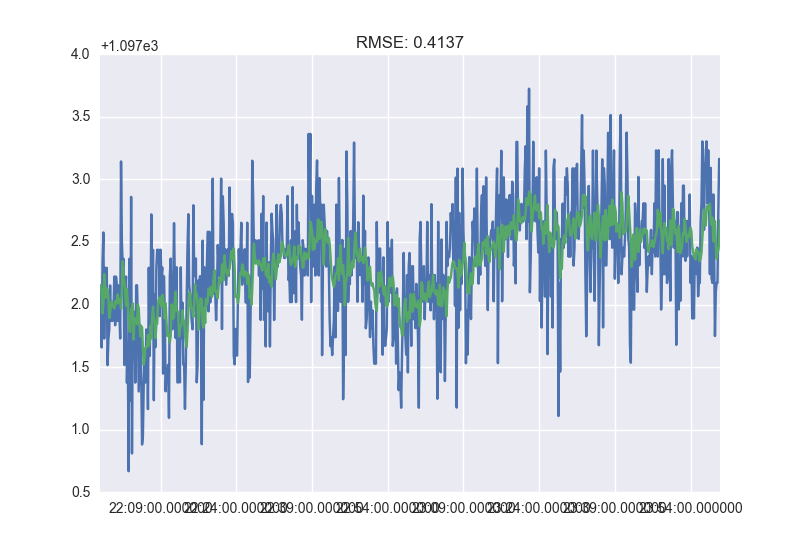
\includegraphics[width=\textwidth]{arima_c1_all_dataset.png}
                \caption{Ajuste ARIMA para la componente 1.}
                \label{fig:arima_c1_all_dataset_fit}
            \end{subfigure}
            \begin{subfigure}[h]{0.49\textwidth}
                \centering
                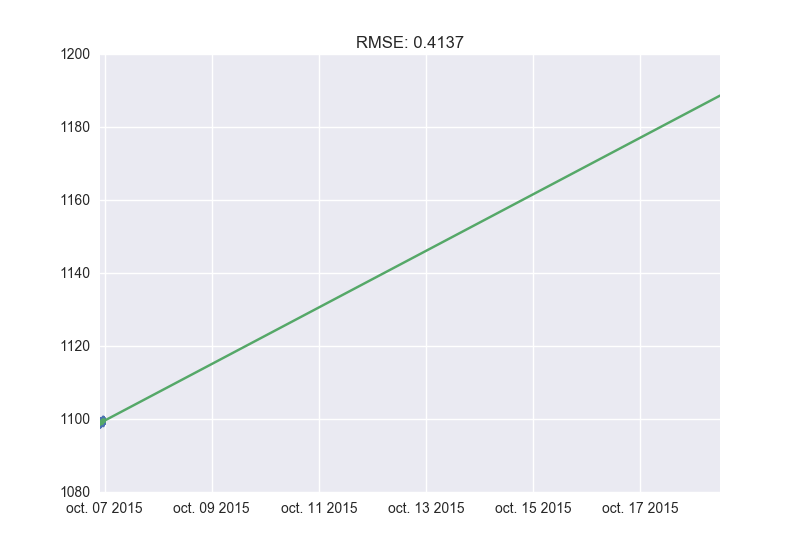
\includegraphics[width=\textwidth]{arima_c1_all_dataset_pred.png}
                \caption{Predicción ARIMA para la componente 1.}
                \label{fig:arima_c1_all_dataset_pred}
            \end{subfigure}
            \caption{ARIMA para la componente 1 calculada con PCA sobre todo el {\em dataset}.}
            \label{fig:arima_c1_all_dataset}
        \end{figure}

        En el gráfico de predicción {\em in-sample} (Figura~\ref{fig:arima_c1_all_dataset_fit}), podemos ver que el modelo se ajusta bastante bien a la serie de la componente. En el gráfico de predicción {\em out-of-sample} ((Figura~\ref{fig:arima_c1_all_dataset_pred})), vemos que los valores siguen una tendencia creciente, que seguirá hasta infinito. 
        
        \subsection{Predicción ARIMA con PCA de un día}
        El cálculo de PCA debe hacerse sobre los datos del día de la serie y no sobre todo el {\em dataset} como visto en la sección anterior. Con esta corrección, los gráficos de predicción ya no se deterioran y tienden para la media de los datos. La  Figura~\ref{fig:arima_c1_one_day_pred} da cuenta de ese efecto - en azul vemos los datos de la componente y en verde la predicción {\em out-of-sample}.
        
        \begin{figure}[H]
            \centering
            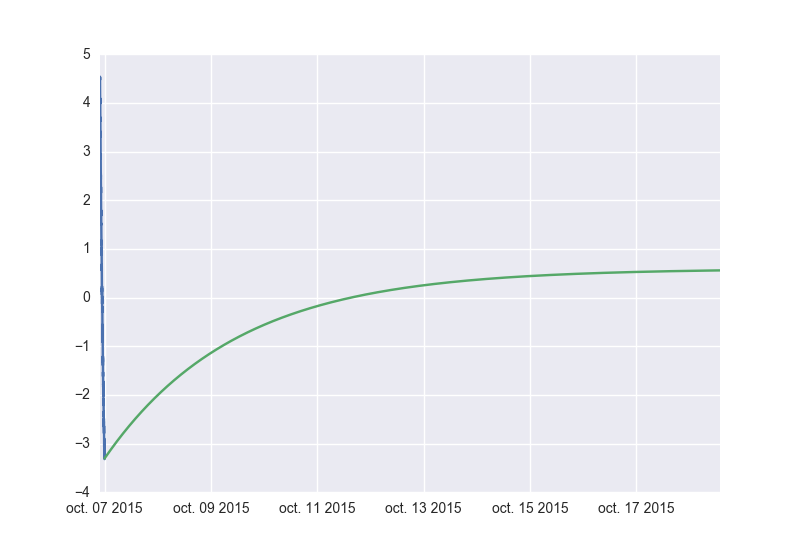
\includegraphics[width=0.7\textwidth]{arima_c1_one_day_pred.png}
            \caption{Predicción {\em out-of-sample} para la componente 1 calculada con PCA de un día.}
            \label{fig:arima_c1_one_day_pred}
        \end{figure}
        
        Los resultados del test \(T^2\) de Hotelling han mejorado con la corrección, asumiendo ahora el estadístico valores más bajos que anteriormente, pero todavía no se puede aceptar la hipótesis de similitud de poblaciones. En la sección siguiente se prueba un nuevo acercamiento al problema.
%        el modelo ARIMA, y cualquier modelo de series temporales, toma como variables explicativas los datos pasados de la misma variable a predecir. Así, estos modelos se activarán cada periodo de tiempo, cogerán los datos pasados y ofrecerán la predicción de un instante más en el futuro de la variable a predecir en cuestión, y esto lo hará tomando como entrada las variables explicativas representadas por los valores de esa variable en el pasado.
        
        \subsection{Simulación con búsqueda de puntos cercanos de la Gaussiana}
        Teniendo en cuenta que la población generada de la simulación ARIMA no pasa el test \(T^2\) de Hotelling, se propone una nueva solución, que se explica a continuación. La solución consiste en generar una simulación de millones de puntos con distribución Gaussiana, que se ha demostrado que es válida. Luego se obtiene un punto simulado con el modelo ARIMA, al cual se añade o no ruido residual, y se busca el punto más cercano a este en los datos Gaussianos. El punto más cercano se usará como representante y se usará para re-alimentar el modelo ARIMA. Luego se procede a generar un nuevo punto en el instante siguiente.
        
        El pseudo-código siguiente explica más secuencialmente la predicción y búsqueda de puntos: 
        \begin{enumerate}
        \item Predicir un valor nuevo para cada componente \(c\) con su respectivo modelo ARIMA. Con esto, para \(N\) componentes, generamos el punto N-dimensional \(p = \{c_{1}, ..., c_{N}\}\). Digamos que tenemos \(N=5\) componentes, entonces el punto sería \(p = \{c_{1}, c_{2}, c_{3}, c_{4}, c_{5}\}\), donde \(c_{x}\) es el valor predicho de cada componente.
        \item (Opcional) Añadir ruido.
        \item Buscar el punto \(p' = \{c_{1}', c_{2}', c_{3}', c_{4}', c_{5}'\}\) más cercano en los puntos de la simulación Gaussiana.
        \item Substituir el punto predicho originalmente \(p\) por \(p'\), en el modelo ARIMA. Con esto, cada \(c_{x}\) es substituído por el \(c_{x}'\) en los datos del modelo ARIMA de cada componente \(c\).
        \item Volver al punto 1.
        \end{enumerate}

En cuanto a distancias puedes probar con la euclídea y la de Mahalanobis y comparar como funcionan ambas.

El tema de comprobar con T2-Hotelling que la simulación gaussiana era coherente con la simulación no era otro que saber que lo que estábamos haciendo tenía sentido y parece que así se constató.

Quizás el problema ahora radica en que si antes la población gaussiana incluía diferentes estados de la máquina y ahora estamos simulando únicamente el último (estacionario), evidentemente no son la misma población, pero eso si es así sería correcto. Pero antes de llegar a ninguna conclusión mejor si lo graficas y vemos que pinta tiene.        
        
         y proyectarlo al espacio natural. Tras esto buscar el punto más cercano (distancia de Mahalanobis) de este punto generado con series a los puntos generados con Gaussiana y quedarnos con ese punto multidimensional más cercano como representante, tras esto este punto será el nuevo punto que usarás para obtener el punto siguiente y procedes de la misma manera comentada anteriormente para el siguiente instante.
        
        El motivo por el que es interesante predecir punto a punto es porque en la simulación vamos a poder simular el punto real del instante una vez busquemos dicho punto en la Gaussiana y parece natural y más realista el cambiar la predicción por la del dato predicho por ARIMA, pues el test T2-Hotelling si que indicaba igualdad de poblaciones, es por ello que tu estimación debería de ser la del punto más próximo dentro de la simulación Gaussiana, con lo que es de esperar que el modelo no se suavice tanto y añada algo de ruido que le de un toque realista a la simulación.

También estaría bien poder hacer esto sin tener que estimar el modelo cada vez, pues eso requiere de un tiempo considerable. Este entrenamiento rutinario te obligaría a ofrecer varias estimaciones de una vez sin poder realimentar el bloque de puntos que predices con nuevos valores. Aunque podrías ir avanzando en paralelo en la parte de la Gaussiana con lo que hay y a la vez ir viendo como solucionar esta parte.

Para la parte de predicción con nuevos valores, a falta de aportar una solución definitiva, se me ocurre que cuando el modelo esté entrenando, entonces hagas una búsqueda exhaustiva de los parámetros del modelo probando con varios AR, I, MA. Pero cuando estés en modo predicción entonces montes el vector con los nuevos datos que adicionarás al final a los anteriores, y hagas la estimación del modelo sin búsqueda exhaustiva de los parámetros AR, I, MA, asignándole los que ya aprendiste durante el training. Operando así, igual podemos llegar a ofrecer una única predicción por instante, pues los tiempos de estimación se deberían de reducir considerablemente.
    
    % Big Data
    \chapter{Big Data}
    TODO
    
        \section{MongoDB}
        TODO
        
        \section{Spark}
        TODO
 
% Conclusiones
\chapter{Conclusiones}
TODO

% Trabajos futuros
\chapter{Trabajos futuros}

ARIMA: añadirle el ruido residual a la predicción y realizar la predicción del siguiente valor con el valor de la predicción actual que incluye el ruido.

\begin{thebibliography}{10}

\bibitem{shlens}
   Jon Shlens.
   \newblock \textit{A TUTORIAL ON PRINCIPAL COMPONENT ANALYSIS. Derivation, Discussion and Singular Value Decomposition.}
   \newblock Version 1, 25 March, 2003.

\bibitem{light}
   Unknown Authors.
   \newblock \textit{The Truth about Principal Components and Factor Analysis.}
   \newblock 28 September, 2009.
   
\bibitem{bishop}
   Christopher M. Bishop.
   \newblock \textit{Pattern Recognition and Machine Learning.}
   \newblock Springer, 2006.

\bibitem{montgomery}
   Montgomery, Douglas C.
   Jennings, Cheryl L.
   Kulahci, Murat
   \newblock \textit{Introduction to Time Series Analysis and Forecasting.}
   \newblock Springer, 2006.

\bibitem{WAR}
   \textit{Principal component analysis (PCA).}
   \newblock Consultar 
   \url{http://scikit-learn.org/stable/modules/decomposition.html#principal-component-analysis-pca}.

\end{thebibliography}
\cleardoublepage

%\APPENDIX
%
%\chapter{Configuración del sistema}
%TODO
%    \section{Fase de inicialización}
%    TODO

\end{document}
